\documentclass{article}
\usepackage{graphicx} % Required for inserti
\usepackage{caption}
\usepackage{subcaption}
\usepackage{geometry}
\usepackage{blindtext}
\usepackage{amsmath}
\usepackage{amsfonts}
\usepackage{amssymb}
\usepackage{tokcycle}
\usepackage{color}
\usepackage{soul}
\usepackage{xcolor}
\usepackage{wrapfig}
\usepackage{pifont}
\usepackage{xifthen}
\usepackage{multirow}
\usepackage{hyperref}
\usepackage{authblk}
\usepackage[numbers]{natbib}
\usepackage{tikz}
\usepackage{pgfplots}
\usepackage{algorithm}
\usepackage{algpseudocode}
\usepackage{scalerel}
\usetikzlibrary{positioning, decorations.pathreplacing,calligraphy, calc, shapes.geometric, intersections, arrows}
\usepgfplotslibrary{fillbetween}
\pgfplotsset{compat=1.18}


\newcommand{\fmri}{functional magnetic resonance imaging}
\newcommand{\FMRI}{Functional magnetic resonance imaging}
\newcommand{\fmriabbrv}{fMRI}
\newcommand{\eeg}{electroencephalography}
\newcommand{\EEG}{Electroencephalography}
\newcommand{\eegabbrv}{EEG}
\newcommand{\correction}[1]{#1}

%\renewcommand{\hl}[1]{#1}

\setcounter{page}{1}

\date{}
\title{EEG to fMRI Synthesis to Aid Medical Decision:\\ A Schizophrenia Case Study}
\author{}

\newtheorem{proposition}{Proposition}
\newtheorem{theorem}{Theorem}
\newtheorem{lemma}{Lemma}
\newtheorem{corollary}{Corollary}
\newtheorem{proof}{Proof}

\begin{document}

\maketitle

\begin{abstract}
Electroencephalography (EEG) captures neuronal activity at the scalp, while functional magnetic resonance imaging (fMRI) provides deeper, spatially rich insights into brain function, though its high cost limits accessibility. EEG-to-fMRI synthesis offers a promising solution, bridging these modalities to enhance diagnostic reach. We propose a framework that leverages both time-frequency (STFT) and synthesized fMRI views to support schizophrenia diagnosis. This is the first study to \hl{evaluate} the clinical potential of EEG-synthesized fMRI, achieving an AUC of $0.77$ and revealing spatial patterns aligned with known biomarkers. The STFT view provides strong predictive accuracy\hl{, AUC of 0.93}, while the fMRI view offers spatial interpretability. Using simultaneous EEG-fMRI data and a novel contrastive loss, we identify \hl{statistically significant} schizophrenia-related patterns in frontal, temporal, and cerebellar regions. \hl{These results position the synthesized fMRI as an interpretable spatial view that localizes dysfunction, with the STFT view carrying the discriminative load, and point toward cost-effective, explainable clinical decision support.}
\end{abstract}

\section{Introduction}\label{section:introduction}

Imagine having access to a high-powered microscope\hl{, e.g. functional magnetic resonance imaging (fMRI),} that reveals the finest details of a complex system, but only at great cost and limited availability. Now, picture a simpler lens, more accessible, portable, and inexpensive, \hl{e.g. electroencephalography (EEG),} though it reveals only the surface. On their own, each tool is limited: one by practicality, the other by depth. But with the power of machine learning, we can bridge this gap, extracting rich information from the cheaper \hl{EEG} lens by learning from the expensive \hl{fMRI} one. \hl{This is what EEG-to-fMRI synthesis is focused on} \cite{calhas2022eeg}. Even if the \hl{EEG} lens cannot match the performance of the high-end tool in isolation, combining their perspectives allows us to make timely, explainable decisions, especially in environments where resources are scarce and speed is essential. \hl{We leverage EEG-to-fMRI synthesis to tackle schizophrenia, a chronic psychiatric disorder characterized by positive symptoms (e.g., hallucinations and delusions), negative symptoms (e.g., affective flattening and avolition), and cognitive impairment, affecting a large global population }\cite{saha2005systematic}\hl{. It is clinically heterogeneous, spanning recognized stages and subtypes, including first-episode psychosis, acute and transient psychotic states, and chronic presentations, that differ in symptom profile and course. Diagnosis remains complex, drawing on psychological, neuroimaging, molecular, and speech-based assessments }\cite{andreou2020structural,neale2015genetic,corcoran2020language}\hl{, which motivates the search for objective, quantitative biomarkers to support it. EEG is a low-cost, portable measure of cortical activity that has yielded numerous markers separating patients with schizophrenia from healthy controls. Complexity and frequency-based descriptors of the EEG further distinguish chronic patients from controls }\cite{tan2016eeg}\hl{.  Beyond stationary spectra, wavelet-domain inter-hemispheric correlations of band activity under affective visual stimulation reveal gamma-band fronto-central alterations in first-episode psychosis }\cite{aydin2018cortical}\hl{, tying emotional processing to measurable EEG signatures. Collectively, these findings establish EEG as an informative, if interpretively limited, window onto schizophrenia-related dysfunction.} fMRI has also shown promise for automated diagnosis \cite{oh2020identifying, velakoulis2006hippocampal, haukvik2013schizophrenia}, its high cost and limited availability, especially in low-resource settings \cite{ogbole2018survey}, limit its use. Recent work in cross-modal synthesis \cite{sikka2018mri,santini2020unpaired,yang2018mri} shows EEG, a cheaper and more portable modality, can approximate fMRI features \cite{abreu2018eeg, daly2019electroencephalography}. EEG-to-fMRI synthesis is emerging as a solution to democratize access to neuroimaging biomarkers.

However, prior work does not address whether these synthesized views are discriminative or interpretable in real-world diagnostic settings \cite{liu2019convolutional, liu2020latent, bricman2021eeg2fmri, calhas2022eeg, mehta2025time, li2024neurobolt, roos2025brainwaves}. We address this gap by demonstrating that synthesized fMRI, generated from EEG alone, can classify schizophrenia with an AUC of $0.77$, offering spatial interpretability that complements the high discriminative power of EEG frequency features. While stft-based features offer strong predictive accuracy, their clinical interpretability remains limited. The synthesized fMRI view offers spatial patterns aligned with known biomarkers, supporting transparent decision-making, even though it is not the stronger classifier. Our synthesized fMRI view aligns with known biomarkers, frontal, temporal, and cerebellar regions, and supports spatial reasoning critical for medical decision-making. To address discriminative power, we employ linear classifiers only to ensure transparent reasoning and easy interpretation, which consequently raises clinical trust levels. Our approach combines a contrastive loss with layer normalization to preserve fMRI style and enable data separation. We benchmark its classification performance and interpretability against raw and time-frequency EEG views. Furthermore, we apply biclustering \cite{govaert2008block} to uncover statistically significant spatial patterns associated with schizophrenia.

\textbf{Key contributions:} (1) Integration of a state-of-the-art EEG-to-fMRI synthesis model for schizophrenia diagnosis; (2) Introduction of a contrastive learning strategy preserving both separability and fMRI structure; (3) Demonstration that synthesized fMRI provides an interpretable spatial view that complements frequency-based EEG features; (4) Identification of \hl{statistically significant} subcortical patterns via biclustering, reinforcing clinical relevance.

\subsection*{Problem description}\label{section:problem_description}  

Let $\mathcal{V} = \{v_1, \dots, v_n\}$ be a set of different views, such that $\forall i \in \{1, \dots, n\}: v_i = \{F_i, \theta_i\}$. A view $v_i$ is characterized by a function structure, $F_i$, and its parameters, $\theta_i$. Each projection $F_i: \mathbb{R}^{D_0} \to \mathbb{R}^{D_i}$ is performed from the original feature space, $\mathbb{R}^{D_0}$, to its view space, $\mathbb{R}^{D_i}$. The original view is defined as $v_0 = \{ I \cdot \vec{x}_0, I \in \mathbb{R}^{D_0}\}$, being $I$ the identity matrix. Each view has a dedicated section, where the structure of its space, $D_i$, is defined. Each instance, $\vec{x}$, is paired with a label $y \in \{0,1\}^K: \sum_k y_k=1$, where $K$ is the number of classes described in the data. A view, $v_i$, optimizes its parameters, $\theta_i$, in order to minimize
\begin{equation}\label{equation:loss}
    \mathcal{L}_C(\vec{x}_0, y) = -y \times \mbox{log}(\sigma(W^i_f \cdot  v_i(\vec{x}_0) + b^i_f)),
\end{equation}
where $W^i_f \in \mathbb{R}^{K \times D_i}$ and $b^i_f \in \mathbb{R}^K$ are the parameters of a linear classifier, referred to as $\theta_C^i = W^i_f \bigcup b^i_f$, using the softmax activation, $\sigma$. Then the objective, for each view $i$, is defined as $\mbox{argmin}_{\theta_C^i} \mathcal{L}_C(\vec{x}_0, y)$.

\section{Background: Defining the EEG views}\label{section:eeg_views}

This study is concerned with providing an accurate view that allows a straightforward interpretation. The interpretation of a decision is typically made by a human being, with knowledge in the application domain \cite{treviso2020explanation}. However, when a prediction is made by a model, it can be supported with explanations, for instance how features $\vec{x}_i$ impact the decision of the model. In this section, we describe each EEG views considered in our experiments, starting with the raw (channel-temporal) view, \textit{raw}, moving to the frequency (channel-time-frequency) representation, referred to as \textit{stft}, and finishing with the synthesized fMRI which is the \textit{fmri} view. For each of these, we discuss their ability to provide good explanations, as well as their overall fit to discriminate schizophrenia.

\subsection{\textit{raw} view}\label{eeg_views:channel_time}

In its raw form, an EEG recording consists of a set of electrodes, also called channels, that contain the electrical activity present at the scalp. This activity has its source at the neurons, where the action potentials occur. Formally this view is defined as $v_0 = \{F_0, \theta_0\}$, where $F_0 = I \cdot \vec{x}_0$ and $\theta_0 = I \in \mathbb{R}^{D_0}$. With EEG being a multivariate time series representation, researchers are able to study functional properties of the brain \cite{huang2020temporal}. However, the application of this specific view is mainly useful for epilepsy detection \cite{tatum2021handbook}. Structurally, this representation is defined as $\vec{x}_0 \in \mathbb{R}^{D_0}$, with $D_0 = C \times T$. $C$ stands for the number of channels and $T$ defines the temporal dimension. It is worth noting that this view is limited to the channel-temporal features, characterized by noise and difficult medical interpretation \cite{de2019introduction}. In consequence, it is unsuitable for diagnosis. In the scope of schizophrenia classification, even when processed by models with a high level of feature engineering \cite{oh2019deep}, it falls short from other more fit views \cite{barros2021advanced}.

\subsection{\textit{stft} view}\label{eeg_views:channel_freq_time}

Research studies, along the years, have had a common trend of extracting time frequency features from the EEG signal. From functional connectivity relations \cite{fingelkurts2007impaired,burgess2002functional,albrecht2018time} to statistical significance of bands associated with pathologies \cite{roach2008event,bates2009low}, several studies have used the frequency domain to uncover new findings. A time frequency representation of EEG can be achieved via a transform \cite{bracewell1986fourier}. In this study we consider the short time Fourier transform (STFT) \cite{jacobsen2003sliding}, whose kernel consists on sine and cosine waves with different shifts and frequencies. As such this view is defined as $v_1=\{F_1, \theta_1\}$, where $F_1$ is the sum of sinusoids and $\theta_1$ are the sinusoids themselves.

Similarly to \textit{raw}, this view is a multivariate time series representation, with the channel, $C$, and temporal, $T$, dimensions belonging to its structure. On top of that, each frequency, with the dimension $F$, is represented at different time steps and channels. Hence, the function consists of $F_1: \mathbb{R}^{D_0} \to \mathbb{R}^{D_1}$ and the \textit{stft} view is structurally defined as $\vec{x}_1 \in \mathbb{R}^{D_1}$, where $D_1 = C \times F \times T$. On the interpretation side, we consider it not just similar to the \textit{raw} view, but also more limited due to the requirement of frequency domain knowledge. Though, its discriminative ability is one of the best for schizophrenia \cite{barros2021advanced}.

\subsection{EEG to fMRI synthesis: \textit{fmri} view}\label{eeg_views:eeg_to_fmri}

\begin{figure*}[!t]
    \centering
    \begin{tikzpicture}
        [inner sep=2mm, scale=0.87]

        \node (x) at (0,0) {};
        
        \node (stft) at ($(x)+(-1.2,0.3)$) {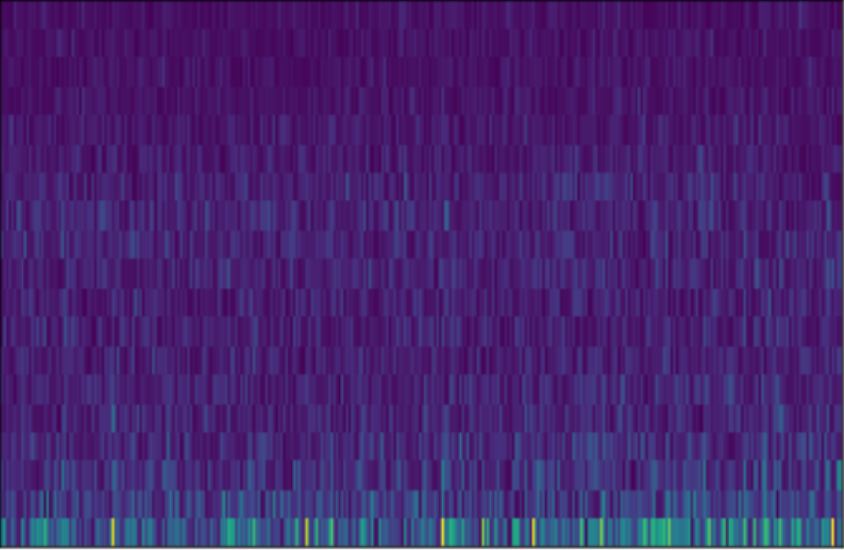
\includegraphics[width=0.1\textwidth]{stft.png}};
        \node (stft) at ($(stft)+(0.1,-0.1)$) {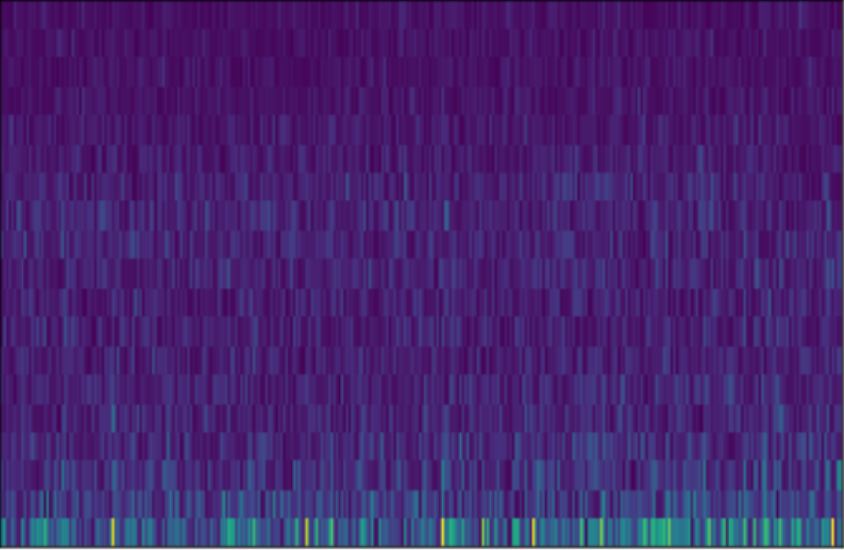
\includegraphics[width=0.1\textwidth]{stft.png}};
        \node (stft) at ($(stft)+(0.1,-0.1)$) {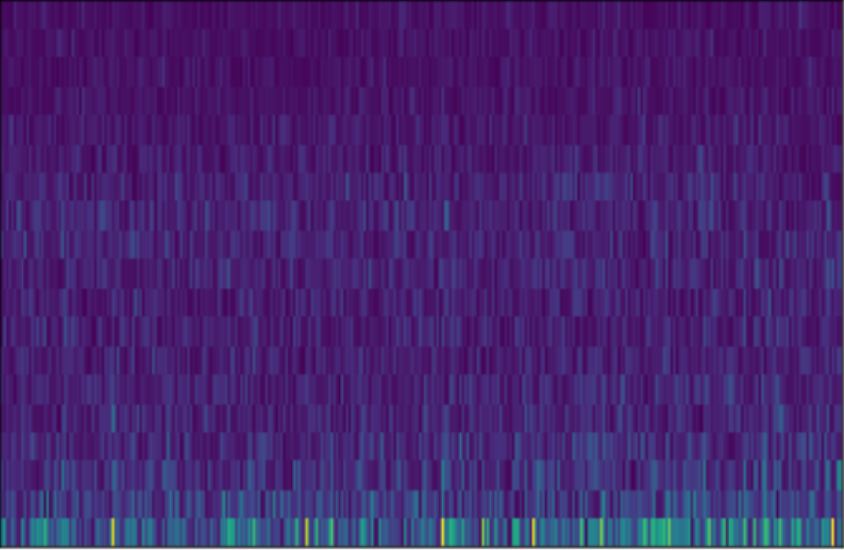
\includegraphics[width=0.1\textwidth]{stft.png}};
        \node (stft) at ($(stft)+(0.1,-0.1)$) {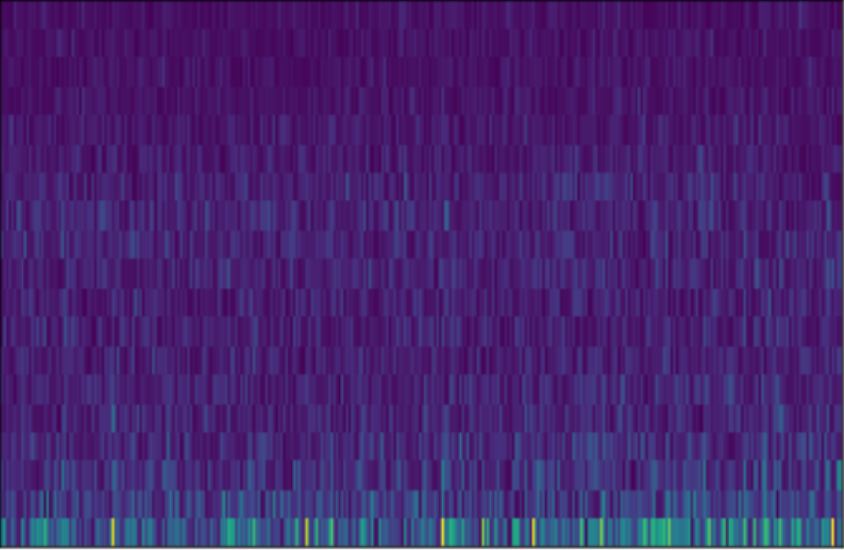
\includegraphics[width=0.1\textwidth]{stft.png}};
        \node (stft) at ($(stft)+(0.1,-0.1)$) {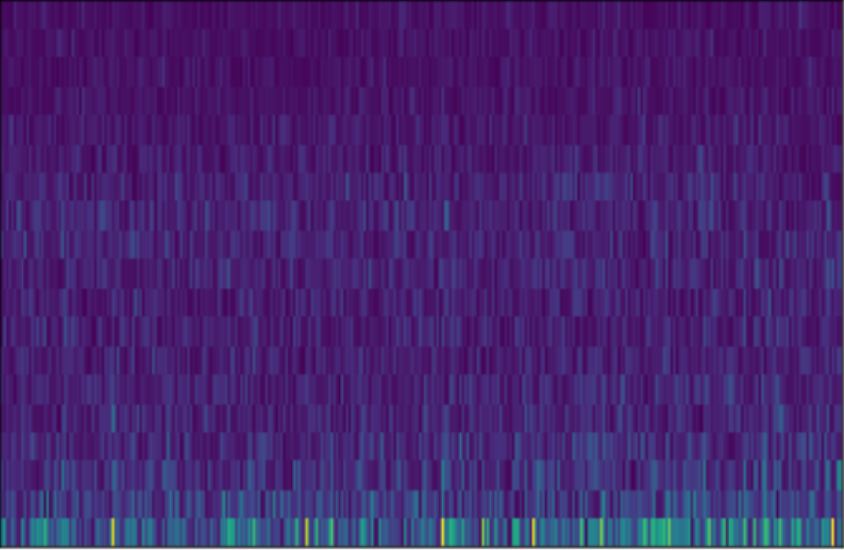
\includegraphics[width=0.1\textwidth]{stft.png}};
        
        \node at ($(stft)+(-0.2,-0.9)$) {$\vec{x}_1$};
        
        \node (encoder) at ($(x)+(2.3,0)$) {\tikz {\draw[rounded corners, draw=black!50,fill=black!20,thick, dash pattern=on 7pt off 2pt] (0,0) rectangle ++(3.4,3);}};
        \node (decoder) at ($(x)+(7.8,0)$) {\tikz {\draw[rounded corners, draw=brown!70,fill=green!20,thick, dash pattern=on 7pt off 2pt] (0,0) rectangle ++(4.5,3);}};
        \node (legend_encoder) at ($(encoder)+(0,-1.9)$) {Encoder};
        \node (legend_decoder) at ($(decoder)+(0,-1.9)$) {Decoder};
        
        
        \node (channel_organization) at ($(x)+(1,0)$) {\tikz {\draw[draw=blue!50,fill=blue!20,thick] (0,0) rectangle ++(0.3,2);}};

        \node (T) at ($(channel_organization)+(0.7,0)$) {$T$};

        \node (resblock1) at ($(T)+(0.7,0)$) {\tikz {\draw[rounded corners, draw=red!40,fill=red!20,thick] (0,0) rectangle ++(0.3,2);}};

        \node (resblock2) at ($(resblock1)+(0.7,0)$) {\tikz {\draw[rounded corners, draw=red!40,fill=red!20,thick] (0,0) rectangle ++(0.3,2);}};

        \node (latent_affine) at ($(resblock2)+(0.7,0)$) {\tikz {\draw[draw=orange!40,fill=orange!20,thick] (0,0) rectangle ++(0.3,2);}};

        \node (latent) at ($(latent_affine)+(1,0)$) {$\vec{z}$};

        \node (fourier) at ($(latent)+(2,0)$) {$cos(\omega \cdot \vec{z} + \beta)$};

        \node (style) at ($(fourier)+(2,0)$) {$\odot $};
        \node (style_weight) at ($(style)+(0,1.3)$) {$W$};

        \node (decoder_affine) at ($(style)+(1,0)$) {\tikz {\draw[draw=orange!40,fill=orange!20,thick] (0,0) rectangle ++(0.3,2);}};

        \node (output) at ($(decoder_affine)+(1.7,0)$) {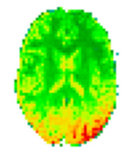
\includegraphics[width=0.1\textwidth]{fmri.png}};
        \node at ($(output)+(0,-1.3)$) {$\vec{x}_2$};
        
        
        \draw[-latex, line width=1pt, black!60] ($(x)+(0.2,0)$) -- ($(channel_organization)+(-0.25,0)$);
        \draw[-latex, line width=1pt, black!60] ($(channel_organization)+(0.2,0)$) -- ($(T)+(-0.2,0)$);
        \draw[-latex, line width=1pt, black!60] ($(T)+(0.2,0)$) -- ($(resblock1)+(-0.2,0)$);
        \draw[-latex, line width=1pt, black!60] ($(resblock1)+(0.2,0)$) -- ($(resblock2)+(-0.2,0)$);
        \draw[-latex, line width=1pt, black!60] ($(resblock2)+(0.2,0)$) -- ($(latent_affine)+(-0.2,0)$);
        \draw[-latex, line width=1pt, black!60] ($(latent_affine)+(0.25,0)$) -- ($(latent)+(-0.25,0)$);
        \draw[-latex, line width=1pt, black!60] ($(latent)+(0.25,0)$) -- ($(fourier)+(-1.25,0)$);
        \draw[-latex, line width=1pt, black!60] ($(fourier)+(1.25,0)$) -- ($(style)+(-0.25,0)$);
        \draw[-latex, line width=1pt, black!60] ($(style)+(0.25,0)$) -- ($(decoder_affine)+(-0.25,0)$);
        \draw[-latex, line width=1pt, black!60] ($(decoder_affine)+(0.25,0)$) -- ($(output)+(-0.8,0)$);
        \draw[-latex, line width=2pt, red!60] ($(style_weight)+(0,-0.25)$) -- ($(style)+(0,0.25)$);
        
        \node (attention_legend) at ($(encoder)+(-3.5,-3.4)$) {\tikz {\draw[draw=blue!50,fill=blue!20,thick] (0,0) rectangle ++(0.3,2);}};
        \node (resblock_legend) at ($(attention_legend)+(2.5,0)$) {\tikz {\draw[rounded corners, draw=red!40,fill=red!20,thick] (0,0) rectangle ++(0.3,2);}};
        \node (affine_legend) at ($(resblock_legend)+(3,0)$) {\tikz {\draw[draw=orange!40,fill=orange!20,thick] (0,0) rectangle ++(0.3,2);}};
        \node (hadamard_legend) at ($(affine_legend)+(3.8,0)$) {$\odot$};

        \node[align=left] at ($(affine_legend)+(1.7,0)$) {Affine projection};
        \node[align=left] at ($(attention_legend)+(1.1,0)$) {Attention};
        \node[align=left] at ($(resblock_legend)+(1.4,0)$) {Resnet block};
        \node at ($(hadamard_legend)+(2.,0)$) {Hadamard product};
        
    \end{tikzpicture}
    \caption{The neural architecture has two components: an Encoder (shaded in grey) and a Decoder (shaded in green). The input is the \textit{stft} $v_1$ representation. The output is the synthesized \textit{fmri}. The Encoder begins with a simple attention mechanism on the channels dimension of the \textit{stft}. After, it is processed by two Resnet blocks and an affine layer. This produces the latent representation $\vec{z}$. Following, the Decoder picks this representation and builds the cosine bases through the projection $\omega \cdot \vec{z} + \beta$. The sinusoids are style induced with $cos(\omega \cdot \vec{z} + \beta)\odot W$. The vector $W$ is a style fixed pretrained vector of an \textit{fmri} representation, learned from a simultaneous EEG and fMRI dataset (described in Section \ref{materials:data}). Finally, an affine layer projects it to the \textit{fmri} space.}
    \label{fig:horizontal_architecture}
\end{figure*}

We now describe an EEG to fMRI synthesis model. \hl{This encoder was introduced and validated against real fMRI in prior work }\cite{calhas2022eeg}\hl{, where, on the NODDI dataset, it achieved an RMSE of $0.3972\pm0.0186$ and an SSIM of $0.4613\pm0.0198$, the best values among the baselines compared therein. We reuse this pretrained mapping here and focus on the downstream diagnostic and interpretive value of the resulting view.} It is a neural network, whose flow is illustrated in Figure \ref{fig:horizontal_architecture}. Its input is the EEG time-frequency representation view, $\vec{x}_1$. On the opposite side, the output is the \textit{fmri} view, $\vec{x}_2 \in \mathbb{R}^{M_1 \times M_2 \times M_3}$, characterized by the referential axes dimensions ($M_1$, $M_2$ and $M_3$). Zooming out of the neural network, we can describe this view as $v_2 = \{ F_2, \theta_2\}$. Where $F_2 = F_1 \bigcup F$ denotes the union of two functions $F_1$, the short time Fourier transform view $v_1 = \{ F_1, \theta_1\}$, and $F$, the neural network. Accordingly, its parameters are $\theta_2 = \theta_1 \bigcup \theta_F$, where $\theta_F$ are the parameters of the neural network. 

In terms of structure, this network processes the input with an attention mechanism. For this, an attention weight matrix $A \in \mathbb{R}^{C \times F \times T}$ is used to compute $E \in \mathbb{R}^{C \times C}$, where $\forall i \in \{1, \dots, C\}: E_i = \begin{bmatrix} e_{i1}^\top, \dots, e_{iC}^\top \end{bmatrix} = \begin{bmatrix} \vec{x}_i^\top \cdot A_1, \dots, \vec{x}_i^\top \cdot A_C \end{bmatrix}$. Then $E$ is softmax normalized, such that 
\begin{align*}
    &\forall i \in \{1, \dots, C\}: \\&B_i^\top = \begin{bmatrix} b_{i1}, \dots, b_{iC}\end{bmatrix} = \begin{bmatrix} \frac{\mbox{exp}(e_1)}{\sum_j \mbox{exp}(e_j)} , \dots, \frac{\mbox{exp}(e_C)}{\sum_j \mbox{exp}(e_j)} \end{bmatrix}.
\end{align*}
Then we can compute the attention processed representation as
\begin{equation}\label{equation:attention_output}
    T_i  = \sum_j^C \vec{x}_i \odot b_{ji}, \forall i \in \{1, \dots, C\}.
\end{equation}
Following, $T$ is processed by a set of $2$ Resnet-18 blocks \cite{he2016deep}, with kernel and stride sizes tuned by a neural architecture search algorithm. These blocks contain a collection of kernels represented by $\theta_k$\footnote{The kernels of the (downsampling) layers are $k_1 \in \mathbb{R}^{7 \times 37 \times 2}$ and $k_2 \in \mathbb{R}^{7 \times 7 \times 2}$. The stride sizes are $3 \times 5 \times 1$ and $2 \times 2 \times 1$, respectively.}. Then, the representation is processed by a fully connected layer. All the parameters until this last layer are referred to as $\theta_E$, which parameterize the encoder of the neural network. After $T$ is processed by the encoder, it is then used to project random Fourier features \cite{rahimi2007random,tancik2020fourier}, parameterized by $\omega$ and $\beta$. Before decoding, the sinudoids are multiplied with a learned latent style vector, $W \in \mathbb{R}^L$, as $\vec{z} \odot W$. The result is processed by an affine transformation, mapping it to the fMRI volume space $\mathbb{R}^{D_2}$. With this, we formulate the function structure $F: \mathbb{R}^{C \times F \times T} \to \mathbb{R}^{D_2}$. \hl{To our knowledge, this is the first study to evaluate EEG-to-fMRI synthesis in a clinical decision-making context, providing new evidence on whether such synthesized views are discriminative and interpretable for diagnosis.}

\section{Adaptation to new data}\label{section:adaptation}

EEG datasets often differ due to variations in experimental setups (e.g., number of channels, sampling frequency, protocol), which affect their representation in $\mathbb{R}^{C \times T}$, where $C$ is the number of channels and $T$ the temporal dimension. Differences in $C$ and $T$ necessitate model adaptation. 
Our neural network requires adjustments when transferring from pretraining to classification datasets, accounting for changes in channel count, electrode layout, sampling rate, and preprocessing. To adapt, we: compute gradients $\nabla_{\theta_C^i} \mathcal{L}C$ for each view, and $\nabla{\theta_E} \mathcal{L}_D$ for $v_2$ to preserve sinusoidal separability; adjust convolutional strides to match latent dimensions; and zero-fill high-frequency components. 
These adaptations are detailed in the following sections. Manual tuning may be needed for datasets beyond those described in Section \ref{section:setting}.

\noindent\textbf{Gradient filtering.}\label{appendix:gradient_filtering} 
The neural network is pretrained on a simultaneous EEG and fMRI dataset. To adapt to an EEG only dataset, the objective minimized is the negative log likelihood,
\begin{equation}\label{equation:nll}
    \mathcal{L}_C(\vec{y}, \hat{y}) = -y \times \mbox{log}(\sigma(\hat{y})),
\end{equation}
\noindent with $\hat{y} = W_f^2 \cdot \vec{x}_2 + b_f^2$ being the logit output which is then processed by the softmax function, $\sigma$. The gradients for $\mathcal{L}_C$ are computed with respect to $\theta_C^i$. This means, all of the weights $\theta_F$ of the neural network, $F$, are trained only $\mathcal{L}_D$, leaving the decoder parameters fixed.

\noindent\textbf{Stride mutation.}\label{appendix:stride_mutation} 
Since there are affine transformations performed in the latent space of the neural network, $F$, the input must be consistent in terms of dimensionality. For this, the neural network can adapt itself by only tweaking the stride size of the initial resnet-18 (convolutional) blocks. This is according to the arithmetic of convolutions, that let us preserve the kernel size (and use the pretrained weights), $k$, and mutate the output dimension, $O$, by changing the stride, $s$, such that $O=\frac{I-k}{s}+1$. For each dataset, one or more blocks of the resnet-18 had its stride size changed so that the latent dimension would match to the pretrained network.

\noindent\textbf{High frequency zero filling.}\label{appendix:high_pass} 
Addressing the third issue, of frequency sample heterogeneity, we propose a high pass filter if the sampling frequency of a new dataset is higher than the one used to pretrain the network (i.e. $> 250$Hz). Since a window of 2 seconds is taken for the STFT, on only needs to apply the high pass filter if needed. In case of a dataset with sampling frequency $< 250$Hz, we propose the use of a Discrete Cosine Transform and add zeroed frequency coefficients to augment the resolution of the signal to $250$Hz.

\section{Methods}\label{section:methods}

\subsection{EEG Preprocessing and Analysis}

\hl{Both datasets provide scalp EEG, acquired with different montages and sampling rates and processed through a common representation pipeline. In the classification dataset (Fribourg }\cite{dataset2022fribourg}\hl{), EEG was recorded with $128$ electrodes placed according to the international $10$--$20$ system at $2048$\,Hz. In the synthesis (pretraining) dataset (NODDI }\cite{dataset_01}\hl{), EEG was recorded simultaneously with fMRI using a $64$-channel MR-compatible system ($10$--$20$ layout) at $250$\,Hz; scanner-induced gradient and ballistocardiographic artifacts were removed following the original release }\cite{dataset_01}\hl{. For both datasets, device, electrode, and artifact-reduction details follow the corresponding source publications }\cite{dataset2022fribourg,dataset_01}\hl{; we analyze the distributed recordings as secondary data and did not re-acquire or re-clean the raw signals. From the cleaned signal we derive the three views used in our experiments (Section }\ref{section:eeg_views}\hl{): the raw channel temporal view $v_0 \in \mathbb{R}^{C \times T}$, the time--frequency view $v_1 \in \mathbb{R}^{C \times F \times T}$ obtained with the short-time Fourier transform (with $2$\,s analysis windows), and the synthesized fMRI view $v_2$ produced by the synthesis network from $v_1$. To reconcile the differing sampling rates across datasets, we apply the adaptation of Section }\ref{section:adaptation}\hl{: a high-pass filter when the sampling frequency exceeds $250$\,Hz (as for Fribourg), and a discrete cosine transform with zero-filled high-frequency coefficients to upsample signals below $250$\,Hz. Each recording is segmented into non-overlapping $20$\,s windows, yielding $12{,}341$ instances for Fribourg and $2{,}296$ for NODDI.}

\subsection{fMRI Data Collection and Analysis} 

\hl{The fMRI modality is present only in the synthesis (pre-training) dataset (NODDI }\cite{dataset_01}\hl{); the classification dataset (Fribourg) is EEG-only and contains no fMRI. In NODDI, fMRI was acquired simultaneously with EEG at rest, with a repetition time (TR) of $2.16$\,s, an echo time (TE) of $30$\,ms, isotropic voxels of $3 \times 3 \times 3$\,mm$^3$, and a volume resolution of $64 \times 64 \times 30$ voxels; full acquisition details follow the original release }\cite{dataset_01}\hl{. These paired EEG--fMRI recordings are used \emph{exclusively} to pre-train the EEG-to-fMRI synthesis network $F$ (Section }\ref{section:eeg_views}\hl{); NODDI carries no diagnostic labels and is never used for classification. At inference no real fMRI is required, as the fMRI view is synthesized from EEG. Accordingly, the fMRI analysis in this work is performed on the \emph{synthesized} volumes $\hat{x}_2$ rather than on acquired scans, in two ways: (i) their discriminative value, through the linear classifier on $v_2$ (Section }\ref{section:validation}\hl{); and (ii) their spatial structure, through biclustering of individuals $\times$ voxels (Section }\ref{setting:biclustering}\hl{), which localizes statistically significant patterns. The reconstruction fidelity of this synthesis model against real held-out fMRI on NODDI was established in prior work }\cite{calhas2022eeg}\hl{ (RMSE $0.3972 \pm 0.0186$, SSIM $0.4613 \pm 0.0198$, best among the compared baselines).}

\subsection{Integration Approach}\label{section:integration}

To fairly compare views, we employ a linear classifier which allowing a direct assessment of representational discriminative power and easy interpretation \cite{treviso2020explanation}.

For the synthesized fMRI view $v_2$, which involves sinusoidal projections, a challenge arises: separation of data via $y|\vec{x}_1$ may be disrupted. Since EEG data inherently contains label-relevant information, preserving the distribution through the sinusoidal transformation is crucial. We address this by ensuring the projection $y|\omega \cdot \vec{z} + \beta$ maintains the same distribution as $y|\vec{x}_2$, enabling effective class separation while preserving sinusoidal structure.

\subsubsection{Sinusoid separation}\label{methods:separation}

\begin{figure}[ht]
    \centering
    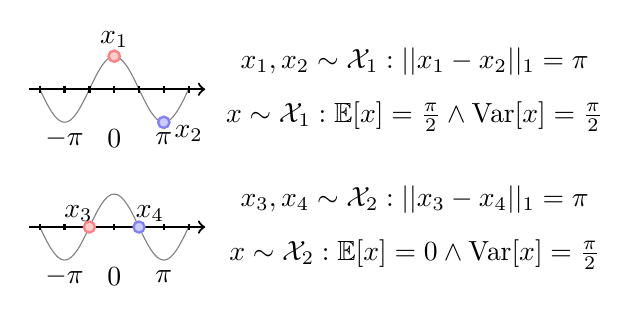
\begin{tikzpicture}
        [scale=0.7,
        inner sep=0.5mm,
        pd/.style={circle,draw=red!50,fill=red!20,thick},
        hc/.style={circle,draw=blue!50,fill=blue!20,thick}]
        
        \node (sinusoid1) at (0,0) {};
        
        \draw[black, thick, ->] ($(sinusoid1)+(-2,0.3)$) -- ($(sinusoid1)+(1.2,0.3)$);%xaxis
        \draw[thin, black!50] ($(sinusoid1)+(0.9,0.3)$) sin ($(sinusoid1)+(0.45,-0.3)$);
        \draw[thin, black!50] ($(sinusoid1)+(0.45,-0.3)$) cos ($(sinusoid1)+(0.,0.3)$);
        \draw[thin, black!50] ($(sinusoid1)+(0.,0.3)$) sin ($(sinusoid1)+(-0.45,0.9)$);
        \draw[thin, black!50] ($(sinusoid1)+(-0.45,0.9)$) cos ($(sinusoid1)+(-0.9,0.3)$);
        \draw[thin, black!50] ($(sinusoid1)+(-0.9,0.3)$) sin ($(sinusoid1)+(-1.35,-0.3)$);
        \draw[thin, black!50] ($(sinusoid1)+(-1.35,-0.3)$) cos ($(sinusoid1)+(-1.8,0.3)$);
        
        
        \draw[black, thick] ($(sinusoid1)+(-1.8,0.36)$) -- ($(sinusoid1)+(-1.8,0.24)$);
        \draw[black, thick] ($(sinusoid1)+(-1.35,0.36)$) -- ($(sinusoid1)+(-1.35,0.24)$);
        \draw[black, thick] ($(sinusoid1)+(-0.9,0.36)$) -- ($(sinusoid1)+(-0.9,0.24)$);
        \draw[black, thick] ($(sinusoid1)+(-0.45,0.36)$) -- ($(sinusoid1)+(-0.45,0.24)$);
        \draw[black, thick] ($(sinusoid1)+(0.,0.36)$) -- ($(sinusoid1)+(0.,0.24)$);
        \draw[black, thick] ($(sinusoid1)+(0.45,0.36)$) -- ($(sinusoid1)+(0.45,0.24)$);
        \draw[black, thick] ($(sinusoid1)+(0.9,0.36)$) -- ($(sinusoid1)+(0.9,0.24)$);
        
        \node at ($(sinusoid1)+(-1.35,-0.6)$) {$-\pi$};
        \node at ($(sinusoid1)+(-0.45,-0.6)$) {$0$};
        \node at ($(sinusoid1)+(0.45,-0.6)$) {$\pi$};
        
        \node (ind1) at ($(sinusoid1)+(-0.45,0.9)$) [pd] {};
        \node (ind1) at ($(sinusoid1)+(0.45,-0.3)$) [hc] {};
        
        \node (ind1) at ($(sinusoid1)+(-0.45,0.9)$) [pd] {};
        \node (ind1) at ($(sinusoid1)+(0.45,-0.3)$) [hc] {};
        
        
        \node (sinusoid2) at ($(sinusoid1)+(0,-2.5)$) {};
        
        \draw[black, thick, ->] ($(sinusoid2)+(-2,0.3)$) -- ($(sinusoid2)+(1.2,0.3)$);%xaxis
        \draw[thin, black!50] ($(sinusoid2)+(0.9,0.3)$) sin ($(sinusoid2)+(0.45,-0.3)$);
        \draw[thin, black!50] ($(sinusoid2)+(0.45,-0.3)$) cos ($(sinusoid2)+(0.,0.3)$);
        \draw[thin, black!50] ($(sinusoid2)+(0.,0.3)$) sin ($(sinusoid2)+(-0.45,0.9)$);
        \draw[thin, black!50] ($(sinusoid2)+(-0.45,0.9)$) cos ($(sinusoid2)+(-0.9,0.3)$);
        \draw[thin, black!50] ($(sinusoid2)+(-0.9,0.3)$) sin ($(sinusoid2)+(-1.35,-0.3)$);
        \draw[thin, black!50] ($(sinusoid2)+(-1.35,-0.3)$) cos ($(sinusoid2)+(-1.8,0.3)$);
        
        
        \draw[black, thick] ($(sinusoid2)+(-1.8,0.36)$) -- ($(sinusoid2)+(-1.8,0.24)$);
        \draw[black, thick] ($(sinusoid2)+(-1.35,0.36)$) -- ($(sinusoid2)+(-1.35,0.24)$);
        \draw[black, thick] ($(sinusoid2)+(-0.9,0.36)$) -- ($(sinusoid2)+(-0.9,0.24)$);
        \draw[black, thick] ($(sinusoid2)+(-0.45,0.36)$) -- ($(sinusoid2)+(-0.45,0.24)$);
        \draw[black, thick] ($(sinusoid2)+(0.,0.36)$) -- ($(sinusoid2)+(0.,0.24)$);
        \draw[black, thick] ($(sinusoid2)+(0.45,0.36)$) -- ($(sinusoid2)+(0.45,0.24)$);
        \draw[black, thick] ($(sinusoid2)+(0.9,0.36)$) -- ($(sinusoid2)+(0.9,0.24)$);
        
        \node at ($(sinusoid2)+(-1.35,-0.6)$) {$-\pi$};
        \node at ($(sinusoid2)+(-0.45,-0.6)$) {$0$};
        \node at ($(sinusoid2)+(0.45,-0.6)$) {$\pi$};
        
        \node (ind1) at ($(sinusoid2)+(-0.9,0.3)$) [pd] {};
        \node (ind1) at ($(sinusoid2)+(0.,0.3)$) [hc] {};
        
        
        \node at ($(sinusoid1)+(-0.45,1.2)$) {$x_1$};
        \node at ($(sinusoid1)+(0.9,-0.5)$) {$x_2$};
        
        \node at ($(sinusoid2)+(-1.1,0.55)$) {$x_3$};
        \node at ($(sinusoid2)+(0.2,0.55)$) {$x_4$};
        
        \node (distance1) at ($(sinusoid1)+(5,0.8)$) {$x_1, x_2 \sim \mathcal{X}_1: ||x_1-x_2||_1=\pi$};
        \node at ($(distance1)+(0,-1)$) {$x \sim \mathcal{X}_1: \mathbb{E}[x] = \frac{\pi}{2} \wedge \mbox{Var}[x]=\frac{\pi}{2}$};
        
        \node (distance2) at ($(sinusoid2)+(5,0.8)$) {$x_3, x_4 \sim \mathcal{X}_2: ||x_3-x_4||_1=\pi$};
        \node at ($(distance2)+(0,-1)$) {$x \sim \mathcal{X}_2: \mathbb{E}[x] = 0 \wedge \mbox{Var}[x]=\frac{\pi}{2}$};
    \end{tikzpicture}
    \caption{Description of how two similarly distributed samples, taken from $\mathcal{X}_1$ and $\mathcal{X}_2$, can lead to different portions of the cosine function image, since a sinusoid is periodic. Two distributions $\mathcal{X}_1$ and $\mathcal{X}_2$, may be mapped to the same image (second/bottom example). This is why a cosine is a shift invariant function. However, there are intervals a shift can be made and it is not invariant. Such intervals take the form $\forall i \in \mathbb{Z}: [i \pi, (i+1)\pi]$.}
    \label{fig:normalization_shift}
\end{figure}

In order to separate data along the projection of cosines, we have to operate in a sub-domain interval where the $cos$ is not periodic. Layer normalization \cite{ba2016layer}, with center in $\frac{\pi}{2}$ and standard deviation of $\frac{\pi}{2}$, maps most of the data to such an interval of the cosine. See Figure \ref{fig:normalization_shift} for an illustration example.

Nonetheless, the assurance that the projections are likely in a non periodic sub-domain of the cosine function, does not alone complete separation of the data. This is because the distribution $y|\omega \cdot \vec{z} +\beta$ needs to be separated accordingly. We propose a modified contrastive loss defined as
\begin{equation}\label{equation:contrastive}
    \mathcal{L}_D(p_1, p_2, y_p) = y_p \times D(p_1, p_2) + (1-y_p) \times ||D(p_1,p_2)-m||_1,
\end{equation}
where $p_1, p_2$ formulate a pair of two instances and $y_p \in \{0,1\}$ defines the pairwise label, being $0$ when the label of $p_1, p_2$ mismatch and $1$ when they match. $D(p_1,p_2)$ is the $l$1 distance $||p_1-p_2||_1^1$. Setting $m\in[\epsilon, \pi]: \epsilon>0$, together with the described layer normalization, allows separation of the data within a non  periodic sub domain of the cosine. 
\begin{theorem}[Separation under Cosine Projection]
Let $z_1, z_2 \in \mathbb{R}^d$ be two latent vectors such that each coordinate lies in $[0, \pi]$. Let the projection be defined as
\[
\phi(z) = \cos(\omega^\top z + \beta),
\]
where $\omega \sim \mathcal{N}(0, I_d)$ and $\beta \sim \mathrm{Uniform}[0, 2\pi]$. Then, for $\|z_1 - z_2\|_2 \geq \epsilon > 0$, the expected cosine similarity between $\phi(z_1)$ and $\phi(z_2)$ satisfies
\[
\mathbb{E}_{\omega, \beta}[\phi(z_1)^\top \phi(z_2)] < d.
\]
Moreover, this expected similarity decreases exponentially with increasing $\|z_1 - z_2\|_2$.
\end{theorem}
The minimization of $\mathcal{L}_D$, together with the described layer normalization, lead to a successful separation of the data when projected by the cosine function. 
\begin{proposition}[Separation under Cosine Projection]
Let $\mathbf{z}_1, \mathbf{z}_2 \in \mathbb{R}^d$ be two latent vectors normalized such that each element lies in the interval $[0, \pi]$. Let $\phi(\mathbf{z}) = \cos(\omega \cdot \mathbf{z} + \beta)$, where $\omega \sim \mathcal{N}(0, I)$ and $\beta$ is a random phase shift. Then, the expected cosine similarity between $\phi(\mathbf{z}_1)$ and $\phi(\mathbf{z}_2)$ is strictly less than 1 if $\|\mathbf{z}_1 - \mathbf{z}_2\| > \epsilon$ for some $\epsilon > 0$. Moreover, separation improves with increased contrastive margin $m$.
\end{proposition}
In Figure \ref{fig:sinusoid_separation}, we illustrate the effects of this methodology, before and after the learning session.

\begin{figure}[ht]
    \centering
    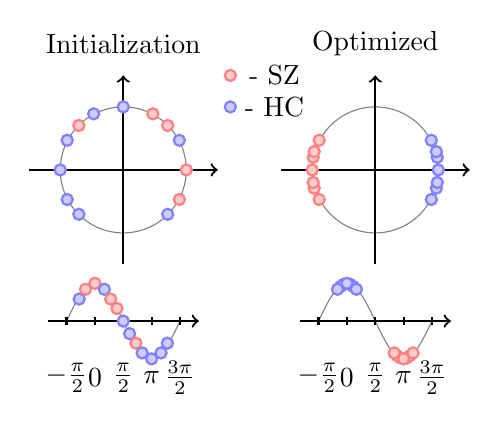
\begin{tikzpicture}
        [scale=0.8,
        inner sep=0.5mm,
        pd/.style={circle,draw=red!50,fill=red!20,thick},
        hc/.style={circle,draw=blue!50,fill=blue!20,thick}]
        
        %draw unit circle
        \node (uni_circle1) at (0,0) {};
        \draw[black!50, thin] ($(uni_circle1)$) circle [radius=1];
        \draw[black, thick, ->] ($(uni_circle1)+(-1.5,0)$) -- ($(uni_circle1)+(1.5,0)$);%xaxis
        \draw[black, thick, ->] ($(uni_circle1)+(0,-1.5)$) -- ($(uni_circle1)+(0,1.5)$);%yaxis
        
        \node (ind1) at ($(uni_circle1)+(1,0)$) [pd] {};
        \node (ind2) at ($(uni_circle1)+(0,1)$) [hc] {};
        \node (ind1) at ($(uni_circle1)+(-0.705,0.705)$) [pd] {};
        \node (ind1) at ($(uni_circle1)+(0.705,0.705)$) [pd] {};
        \node (ind1) at ($(uni_circle1)+(0.47,0.89)$) [pd] {};
        \node (ind2) at ($(uni_circle1)+(-1,0)$) [hc] {};
        \node (ind2) at ($(uni_circle1)+(-0.89,-0.47)$) [hc] {};
        \node (ind2) at ($(uni_circle1)+(-0.705,-0.705)$) [hc] {};
        \node (ind2) at ($(uni_circle1)+(0.89,0.47)$) [hc] {};
        \node (ind2) at ($(uni_circle1)+(-0.89,0.47)$) [hc] {};
        \node (ind2) at ($(uni_circle1)+(-0.47,0.89)$) [hc] {};
        \node (ind2) at ($(uni_circle1)+(0.89,-0.47)$) [pd] {};
        \node (ind2) at ($(uni_circle1)+(0.705,-0.705)$) [hc] {};
        
        
        \node (legend) at ($(uni_circle1)+(1.7,1)$) {};
        \node at ($(legend)+(0.7,0.5)$) {- SZ};
        \node at ($(legend)+(0.7,0)$) {- HC};
        \node at ($(legend)+(0,0.5)$) [pd] {};
        \node at ($(legend)+(0,0)$) [hc] {};
        
        %draw unit circle
        \node (uni_circle2) at ($(uni_circle1)+(4,0)$) {};
        \draw[black!50, thin] ($(uni_circle2)$) circle [radius=1];
        \draw[black, thick, ->] ($(uni_circle2)+(-1.5,0)$) -- ($(uni_circle2)+(1.5,0)$);%xaxis
        \draw[black, thick, ->] ($(uni_circle2)+(0,-1.5)$) -- ($(uni_circle2)+(0,1.5)$);%yaxis
        
        
        %individuals
        \node (ind1) at ($(uni_circle2)+(-1,0)$) [pd] {};
        \node (ind1) at ($(uni_circle2)+(-0.89,0.47)$) [pd] {};
        \node (ind1) at ($(uni_circle2)+(-0.985,0.2)$) [pd] {};
        \node (ind1) at ($(uni_circle2)+(-0.97,0.29)$) [pd] {};
        \node (ind1) at ($(uni_circle2)+(-0.89,-0.47)$) [pd] {};
        \node (ind1) at ($(uni_circle2)+(-0.97,-0.29)$) [pd] {};
        \node (ind1) at ($(uni_circle2)+(-0.985,-0.2)$) [pd] {};
        
        \node (ind2) at ($(uni_circle2)+(1,0)$) [hc] {};
        \node (ind1) at ($(uni_circle2)+(0.89,0.47)$) [hc] {};
        \node (ind1) at ($(uni_circle2)+(0.985,0.2)$) [hc] {};
        \node (ind1) at ($(uni_circle2)+(0.97,0.29)$) [hc] {};
        \node (ind1) at ($(uni_circle2)+(0.89,-0.47)$) [hc] {};
        \node (ind1) at ($(uni_circle2)+(0.97,-0.29)$) [hc] {};
        \node (ind1) at ($(uni_circle2)+(0.985,-0.2)$) [hc] {};
        
        
        
        \node (sinusoid1) at ($(uni_circle1)+(0,-2.7)$) {};
        \draw[black, thick, ->] ($(sinusoid1)+(-1.2,0.3)$) -- ($(sinusoid1)+(1.2,0.3)$);%xaxis
        \draw[thin, black!50] ($(sinusoid1)+(0.9,0.3)$) sin ($(sinusoid1)+(0.45,-0.3)$);
        \draw[thin, black!50] ($(sinusoid1)+(0.45,-0.3)$) cos ($(sinusoid1)+(0.,0.3)$);
        \draw[thin, black!50] ($(sinusoid1)+(0.,0.3)$) sin ($(sinusoid1)+(-0.45,0.9)$);
        \draw[thin, black!50] ($(sinusoid1)+(-0.45,0.9)$) cos ($(sinusoid1)+(-0.9,0.3)$);
        
        \draw[black, thick] ($(sinusoid1)+(-0.9,0.36)$) -- ($(sinusoid1)+(-0.9,0.24)$);
        
        \draw[black, thick] ($(sinusoid1)+(-0.45,0.36)$) -- ($(sinusoid1)+(-0.45,0.24)$);
        \draw[black, thick] ($(sinusoid1)+(0.,0.36)$) -- ($(sinusoid1)+(0.,0.24)$);
        \draw[black, thick] ($(sinusoid1)+(0.45,0.36)$) -- ($(sinusoid1)+(0.45,0.24)$);
        \draw[black, thick] ($(sinusoid1)+(0.9,0.36)$) -- ($(sinusoid1)+(0.9,0.24)$);
        
        \node at ($(sinusoid1)+(-0.9,-0.6)$) {$-\frac{\pi}{2}$};
        \node at ($(sinusoid1)+(-0.45,-0.6)$) {$0$};
        \node at ($(sinusoid1)+(0.,-0.6)$) {$\frac{\pi}{2}$};
        \node at ($(sinusoid1)+(0.45,-0.6)$) {$\pi$};
        \node at ($(sinusoid1)+(0.9,-0.6)$) {$\frac{3\pi}{2}$};
        
        \node (ind1) at ($(sinusoid1)+(-0.7,0.65)$) [hc] {};
        \node (ind1) at ($(sinusoid1)+(-0.6,0.805)$) [pd] {};
        \node (ind1) at ($(sinusoid1)+(-0.45,0.9)$) [pd] {};
        \node (ind1) at ($(sinusoid1)+(-0.3,0.805)$) [hc] {};
        \node (ind1) at ($(sinusoid1)+(-0.2,0.65)$) [pd] {};
        \node (ind1) at ($(sinusoid1)+(-0.1,0.5)$) [pd] {};
        \node (ind1) at ($(sinusoid1)+(0.,0.3)$) [hc] {};
        \node (ind1) at ($(sinusoid1)+(0.1,0.1)$) [hc] {};
        \node (ind1) at ($(sinusoid1)+(0.2,-0.05)$) [pd] {};
        \node (ind1) at ($(sinusoid1)+(0.3,-0.205)$) [hc] {};
        \node (ind1) at ($(sinusoid1)+(0.45,-0.3)$) [hc] {};
        \node (ind1) at ($(sinusoid1)+(0.6,-0.205)$) [hc] {};
        \node (ind1) at ($(sinusoid1)+(0.7,-0.05)$) [hc] {};
        
        \node (sinusoid2) at ($(uni_circle2)+(0,-2.7)$) {};
        \draw[black, thick, ->] ($(sinusoid2)+(-1.2,0.3)$) -- ($(sinusoid2)+(1.2,0.3)$);%xaxis
        \draw[thin, black!50] ($(sinusoid2)+(0.9,0.3)$) sin ($(sinusoid2)+(0.45,-0.3)$);
        \draw[thin, black!50] ($(sinusoid2)+(0.45,-0.3)$) cos ($(sinusoid2)+(0.,0.3)$);
        \draw[thin, black!50] ($(sinusoid2)+(0.,0.3)$) sin ($(sinusoid2)+(-0.45,0.9)$);
        \draw[thin, black!50] ($(sinusoid2)+(-0.45,0.9)$) cos ($(sinusoid2)+(-0.9,0.3)$);
        
        \draw[black, thick] ($(sinusoid2)+(-0.9,0.36)$) -- ($(sinusoid2)+(-0.9,0.24)$);
        
        \draw[black, thick] ($(sinusoid2)+(-0.45,0.36)$) -- ($(sinusoid2)+(-0.45,0.24)$);
        \draw[black, thick] ($(sinusoid2)+(0.,0.36)$) -- ($(sinusoid2)+(0.,0.24)$);
        \draw[black, thick] ($(sinusoid2)+(0.45,0.36)$) -- ($(sinusoid2)+(0.45,0.24)$);
        \draw[black, thick] ($(sinusoid2)+(0.9,0.36)$) -- ($(sinusoid2)+(0.9,0.24)$);
        
        \node at ($(sinusoid2)+(-0.9,-0.6)$) {$-\frac{\pi}{2}$};
        \node at ($(sinusoid2)+(-0.45,-0.6)$) {$0$};
        \node at ($(sinusoid2)+(0.,-0.6)$) {$\frac{\pi}{2}$};
        \node at ($(sinusoid2)+(0.45,-0.6)$) {$\pi$};
        \node at ($(sinusoid2)+(0.9,-0.6)$) {$\frac{3\pi}{2}$};
        
        
        \node (ind1) at ($(sinusoid2)+(-0.5,0.885)$) [hc] {};
        \node (ind1) at ($(sinusoid2)+(-0.55,0.85)$) [hc] {};
        \node (ind1) at ($(sinusoid2)+(-0.6,0.805)$) [hc] {};
        \node (ind1) at ($(sinusoid2)+(-0.4,0.885)$) [hc] {};
        \node (ind1) at ($(sinusoid2)+(-0.35,0.85)$) [hc] {};
        \node (ind1) at ($(sinusoid2)+(-0.3,0.805)$) [hc] {};
        \node (ind1) at ($(sinusoid2)+(-0.45,0.9)$) [hc] {};
        
        
        \node (ind1) at ($(sinusoid2)+(0.5,-0.285)$) [pd] {};
        \node (ind1) at ($(sinusoid2)+(0.55,-0.25)$) [pd] {};
        \node (ind1) at ($(sinusoid2)+(0.6,-0.205)$) [pd] {};
        \node (ind1) at ($(sinusoid2)+(0.4,-0.285)$) [pd] {};
        \node (ind1) at ($(sinusoid2)+(0.35,-0.25)$) [pd] {};
        \node (ind1) at ($(sinusoid2)+(0.3,-0.205)$) [pd] {};
        \node (ind1) at ($(sinusoid2)+(0.45,-0.3)$) [pd] {};
        
        \node (title1) at ($(uni_circle1)+(0,2)$) {Initialization};
        \node (title2) at ($(uni_circle2)+(0,2)$) {Optimized};
        
        %\node (stats1) at ($(uni_circle1)+(0,-4)$) {$\mathbb{E}[f_x(x)]=\frac{\pi}{2}, \mbox{Var}[f_x(x)]=\frac{\pi}{2}$};
        %\node (stats2) at ($(uni_circle2)+(0,-4)$) {$\mathbb{E}[f_x(x)]=\frac{\pi}{2}, \mbox{Var}[f_x(x)]=\frac{\pi}{2}$};
        
    \end{tikzpicture}
    \caption{Normalization of data points inside the unit circle, using layer normalization, along with the optimization of a contrastive loss lead to correct separation of sinusoids. Data points belong to two classes, $HC$ and $SZ$, that are separated after the minimization of $\mathcal{L}_D$. Because we separate false pairs, according to $(1-y_p) \times ||D(x_1,x_2)-m||_1$, all points are placed within a shift variant interval of the cosine. The variance needed for classification.}
    \label{fig:sinusoid_separation}
\end{figure}


\subsection{Dataset Characteristics}\label{materials:data}

\hl{Table }\ref{tab:data_description}\hl{ summarizes both datasets and their distinct roles. The Fribourg dataset }\cite{dataset2022fribourg}\hl{ is the sole classification cohort: $43$ participants ($24$ healthy controls and $19$ patients with a schizophrenia-spectrum (psychotic) disorder), recorded during a task-based session, the Ultimatum Game, played in both proposer and responder roles over three blocks of $30$ repetitions each. Patients were diagnosed clinically according to ICD-10 criteria through the Fribourg Mental Health Network (RFSM); the study was approved under ethics reference $054/13$-CER-FR. The public release distributes the diagnostic group label but not per-subject demographics: age, sex, symptom-severity scales, and illness duration are not included in the distributed data, and group-level characteristics are reported in the associated cohort publication }\cite{horat2018impaired}\hl{.}

\begin{table}[t]
    \centering
    \caption{\hl{Characteristics and distinct roles of the two datasets.}}
    \label{tab:data_description}
    \begin{tabular}{p{3.9cm} | p{4.9cm} | p{5cm} }
        \hline
        \hline
         \hfil & \hfil \hl{Fribourg} & \hfil \hl{NODDI} \\
         \hline
         \hfil \hl{Role} & \hfil \hl{Schizophrenia classification} & \hfil \hl{Pretrain EEG-to-fMRI synthesis}  \\
         \hfil \hl{Paradigm} & \hfil \hl{Task-based (Ultimatum Game)} & \hfil \hl{Resting state} \\
         \hfil \hl{Subjects (total)} & \hfil \hl{43} & \hfil \hl{17} \\
         \hfil \hl{Group balance (HC/SZ)} & \hfil \hl{24/19} & \hfil \hl{n/a (no diagnostic labels used)} \\
         \hfil \hl{Sex (M / F)} & \hfil \hl{23/20} & \hfil \hl{11/6} \\
         \hfil \hl{Age (mean $\pm$ std)} & \hfil \small{\hl{$26.62 \pm 4.91$ SZ $ 24.77 \pm 3.70$ HC}} & \hfil \hl{$32.84 \pm 8.13$} \\
         \hfil \hl{Illness duration} & \hfil \hl{Not available (NA)} & \hfil \hl{not applicatble (n/a)} \\
         \hfil \hl{Diagnostic criteria} & \hfil \hl{ICD-10} & \hfil \hl{n/a} \\
         \hfil \hl{EEG channels} & \hfil \hl{128 (10-20 system)} & \hfil \hl{64 (10-20 system)} \\
         \hfil \hl{Sampling rate} & \hfil \hl{2048 Hz} & \hfil \hl{250 Hz} \\
         \hfil \hl{EEG device} & \hfil \hl{NeuroSpec Quick Cap} & \hfil \hl{BrainCap MR} \\
         \hfil \hl{Windowing / instances} & \hfil \hl{20 s windows; 12,341 instances} & \hfil \hl{20 s windows; 2,296 instances} \\
         \hfil \hl{Ethics approval} & \hfil \hl{054/13-CER-FR} & \hfil \hl{ID:4290/001} \\
         \hline
         \hline
    \end{tabular}
\end{table}

\hl{The NODDI dataset {\cite{dataset_01}} is used only to pre-train the synthesis model and carries no diagnostic labels. It comprises $17$ participants (M/F $= 11/6$; age $32.84 \pm 8.13$ years), recorded at rest with simultaneous EEG and fMRI under ethics reference $4290/001$. Both datasets are previously published, anonymized releases analyzed here as secondary data; behavioural responses for the Ultimatum Game are not available in the public Fribourg release.}


\section{Experimental setting}\label{section:setting}\vskip0.2cm

\begin{figure*}[ht]
    \centering
    \begin{tikzpicture}
        [scale=1.0, inner sep=2mm]

        \node (loop) at (0,0) [draw,rounded corners,thick,white,minimum width=200,minimum height=60] {};

        \node at ($(loop.west)+(-0.6,3)$) {Loop phase};
        \node[align=right] at ($(loop.west)+(-0.9,0)$){For each $s\in S:$};
        \node (ind_out) at ($(loop)+(-2.7,0.7)$) {}; 
        

        %eeg view
        \node (stft) at ($(ind_out)+(3,-0.59)$) {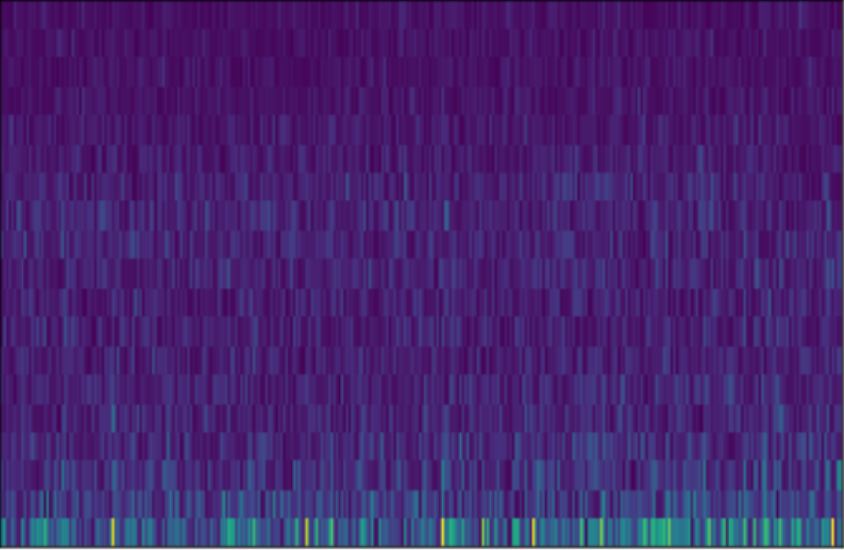
\includegraphics[width=0.07\textwidth]{stft.png}};

        \node (raw) [anchor=south] at ($(stft.north)+(0.,0.7)$) {\includegraphics[width=0.07\textwidth]{eeg.png}};
        
        %fmri
        \node (fmri) [anchor=north] at ($(stft.south)+(0,-0.5)$) {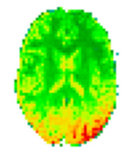
\includegraphics[width=0.07\textwidth]{fmri.png}};
        
        \node (loop_rectangle) [anchor=west] at ($(loop)+(-3.1,0)$) [draw,opacity=0.4,rounded corners,thick,orange,fill=orange!20,minimum width=130,minimum height=180] {};

        \node at ($(ind_out)+(0,-1.7)$) {$s$};
        \draw ($(ind_out)$) circle (0.15);
        \draw ($(ind_out)+(0,-0.15)$) -- ($(ind_out)+(-0.2,-0.5)$);
        \draw ($(ind_out)+(0,-0.15)$) -- ($(ind_out)+(0.2,-0.5)$);
        \draw ($(ind_out)+(0,-0.15)$) -- ($(ind_out)+(0,-0.6)$);
        \draw ($(ind_out)+(0,-0.6)$) -- ($(ind_out)+(0.2,-1.)$);
        \draw ($(ind_out)+(0,-0.6)$) -- ($(ind_out)+(-0.2,-1.)$);

        \node (raw_rect) at (raw) [draw,rounded corners,thick,black,minimum width=35,minimum height=35] {};
        \node (stft_rect) at (stft) [draw,rounded corners,thick,cyan,minimum width=35,minimum height=35] {};
        \node (fmri_rect) at (fmri) [draw,rounded corners,thick,magenta,minimum width=35,minimum height=35] {};

        \node [anchor=south] at ($(raw.north)+(0,-0.16)$) {$v_0$ raw};
        \node [anchor=south] at ($(stft.north)+(0,-0.1)$) {$v_1$ stft};
        \node [anchor=north] at ($(fmri.south)+(0,0.325)$) {$v_2$ fmri};

        %\node at ($(raw_rect.north)+(0,0.2)$) {$v_0$};
        %\node at ($(stft_rect.north)+(0,0.2)$) {$v_1$};
        %\node at ($(fmri_rect.north)+(0,0.2)$) {$v_2$};


        \draw[->, black, ultra thick] ($(ind_out.east)+(0.3,-0.5)$) -- (raw.west);
        \draw[->, black, ultra thick] ($(ind_out.east)+(0.3,-0.6)$) -- (stft.west);
        \draw[->, black, ultra thick] ($(ind_out.east)+(0.3,-0.7)$) -- (fmri.west);
        %\draw[->, black, ultra thick] (raw.east) -- (stft.west);
        %\draw[->, black, ultra thick] (stft.east) -- (fmri.west);

        \node (cv) at ($(loop.east)+(-3.5,0)$) [anchor=west, draw,rounded corners,thick,opacity=0,white,minimum width=200,minimum height=60] {};

        \node (cv_rectangle) at (cv) [draw,rounded corners,thick,opacity=0.5,blue,fill=blue!50,minimum width=80,minimum height=180] {};

        \node (net1) at ($(cv)+(-0.6,1.99)$) {};
        \node (net2) at ($(cv)+(-0.6,0.11)$) {};
        \node (net3) at ($(cv)+(-0.6,-1.76)$) {};

        \node[circle,draw=black, fill=white, inner sep=0.3,minimum size=3] (1st_node) at ($(net1)+(0,0.3)$) {};
        \node[circle,draw=black, fill=white, inner sep=0.3,minimum size=3] (2nd_node) at ($(net1)+(0,-0.1)$) {};
        \node[circle,draw=black, fill=white, inner sep=0.3,minimum size=3] (3rd_node) at ($(net1)+(0,0.1)$) {};
        \node[circle,draw=black, fill=white, inner sep=0.3,minimum size=3] (4th_node) at ($(net1)+(0,-0.3)$) {};
        \node[circle,draw=black, fill=white, inner sep=0.3,minimum size=3] (out_node) at ($(net1)+(1,0)$) {};
        \draw (1st_node.east) -- (out_node.west);
        \draw (2nd_node.east) -- (out_node.west);
        \draw (3rd_node.east) -- (out_node.west);
        \draw (4th_node.east) -- (out_node.west);
        \node at ($(out_node.east)+(.20,0)$) {$\hat{y}_0$};


        \node[circle,draw=black, fill=white, inner sep=0.3,minimum size=3] (1st_node) at ($(net2)+(0,0.3)$) {};
        \node[circle,draw=black, fill=white, inner sep=0.3,minimum size=3] (2nd_node) at ($(net2)+(0,-0.1)$) {};
        \node[circle,draw=black, fill=white, inner sep=0.3,minimum size=3] (3rd_node) at ($(net2)+(0,0.1)$) {};
        \node[circle,draw=black, fill=white, inner sep=0.3,minimum size=3] (4th_node) at ($(net2)+(0,-0.3)$) {};
        \node[circle,draw=black, fill=white, inner sep=0.3,minimum size=3] (out_node) at ($(net2)+(1,0)$) {};
        \draw (1st_node.east) -- (out_node.west);
        \draw (2nd_node.east) -- (out_node.west);
        \draw (3rd_node.east) -- (out_node.west);
        \draw (4th_node.east) -- (out_node.west);
        \node at ($(out_node.east)+(.20,0)$) {$\hat{y}_1$};


        \node[circle,draw=black, fill=white, inner sep=0.3,minimum size=3] (1st_node) at ($(net3)+(0,0.3)$) {};
        \node[circle,draw=black, fill=white, inner sep=0.3,minimum size=3] (2nd_node) at ($(net3)+(0,-0.1)$) {};
        \node[circle,draw=black, fill=white, inner sep=0.3,minimum size=3] (3rd_node) at ($(net3)+(0,0.1)$) {};
        \node[circle,draw=black, fill=white, inner sep=0.3,minimum size=3] (4th_node) at ($(net3)+(0,-0.3)$) {};
        \node[circle,draw=black, fill=white, inner sep=0.3,minimum size=3] (out_node) at ($(net3)+(1,0)$) {};
        \draw (1st_node.east) -- (out_node.west);
        \draw (2nd_node.east) -- (out_node.west);
        \draw (3rd_node.east) -- (out_node.west);
        \draw (4th_node.east) -- (out_node.west);
        \node at ($(out_node.east)+(.20,0)$) {$\hat{y}_2$};

        \draw[->, black, ultra thick] ($(raw.east)+(0.1,0.)$) -- ($(raw.east)+(1.75,0.)$);
        \draw[->, cyan, ultra thick] ($(stft.east)+(0.1,0.)$) -- ($(stft.east)+(1.75,0.)$);
        \draw[->, magenta, ultra thick] ($(fmri.east)+(0.1,0.)$) -- ($(fmri.east)+(1.75,0.)$);

        \node at ($(cv_rectangle.south)+(0,-0.4)$) {$argmin_{\theta_C^i} \mathcal{L}_C(\vec{x}_{0},y|S \backslash s)$};

        \node (cv_legend) at ($(cv_rectangle.north)+(0,0.71)$) {Classification phase};
        \node at ($(loop_rectangle.north)+(0,0.71)$) {Feature extraction phase};

        
    \end{tikzpicture}
    \caption{We do a leave-one-individual-out validation, where for each fold we either train a linear classifier with \textit{raw}, \textit{stft} or \textit{fmri} representations. Each representation has its own validation. The arrows inside the feature extraction phase indicate dependency, that is: an \textit{fmri} representation needs an \textit{stft}; \textit{stft} needs the \textit{raw}; and the \textit{raw}, of course, needs an individual's recording, denoted with a human figure. For each fold, $s \in S$, we train a linear classifier without $s$, $argmin_{\theta_C^i} \mathcal{L}_C(\vec{x}_{0},y|S \backslash s)$. In addition, the \textit{fmri} setting also optimizes $argmin_{\theta_E} \mathcal{L}_D$. For all individuals/folds the predictions are saved to compute the area under the curve (AUC) against the ground truth.}
    \label{fig:loocv_classification_compact}
\end{figure*}

The experiments consider 3 EEG views: 1) natural/raw EEG view in $\mathbb{R}^{C \times T}$, referred to as $v_0$; 2) time-frequency representation of EEG in $\mathbb{R}^{C \times F \times T}$, referred to as $v_1$; 3) synthesized fMRI representation in $\mathbb{R}^{M_1 \times M_2 \times M_3}$, referred to as $v_2$. The optimization of the parameters, of each of these, consists on the minimization of $\mathcal{L}_C$, such that the gradients are $\nabla_{\theta_C^i} \mathcal{L}_C$. The special case $v_2=\{F_2, \theta_2\}$ requires a pretraining session in a simultaneous EEG and fMRI dataset, so it learns fMRI representations. Following, comes the minimization of the classification objective, where $\nabla_{\theta_C^2} \mathcal{L}_C$ is computed along with $\nabla_{\theta_E} \mathcal{L}_D$, being $\theta_E$ the parameters of the encoder of $F$ (recall Section \ref{eeg_views:eeg_to_fmri}). All these objectives require the respective data for the computation of the gradients described above. Namely EEG data for classification and, in particular for $v_2$, the simultaneous EEG and fMRI data, for EEG to fMRI synthesis. All experiments were made on a NVIDIA GeForce RTX \hl{2080} GPU (8GB).

\begin{table*}[t]
    \centering
    \caption{Fribourg dataset AUC of a linear classifier, on a LOOCV schema, with different views as input.}
    \begin{tabular}{ p{2cm} | p{2.cm} | p{2.cm} | p{2.cm} | p{2.cm}}
        \hline
        \hline
        \hfil View & \hfil AUC & \hfil Accuracy & \hfil Sensitivity & \hfil Specificity \\
        \hline
            \hfil \textit{raw} $v_0$ & \hfil $0.225$ & \hfil $0.497$ & \hfil $0.037$ & \hfil $0.860$\\
            \hfil \textit{stft} $v_1$ & \hfil $\mathbf{0.933}$ & \hfil $\mathbf{0.891}$ & \hfil $\mathbf{0.832}$ & \hfil $\mathbf{0.936}$\\
            \hfil \textit{fmri} $v_2$ & \hfil $0.765$ & \hfil $0.703$ & \hfil $0.666$ & \hfil $0.733$\\
        \hline
        \hline
    \end{tabular}
    
    \label{tab:auc_schizophrenia}
\end{table*}


\subsection{Validation}\label{section:validation}


To validate each view $v_i$, we perform: 1) leave-one-individual-out cross-validation (LOOCV); 2) 5-fold cross-validation for hyperparameter tuning with 25 iterations per LOOCV fold; 3) for $v_2$, a pretraining of $F$ on simultaneous EEG-fMRI data. Hyperparameters for $F$ follow \cite{calhas2022eeg}; Bayesian optimization \cite{snoek2012practical} tunes: $l1 \in [1\mbox{e}-10, 2.0]$, learning rate $\in [1\mbox{e}-5, 1.0]$, and batch size $\in {1,2,4,8,16,32}$. Training runs for 10 epochs using Adam \cite{kingma2014adam}.\footnote{Code: \url{https://anonymous.4open.science/r/eeg-to-fmri-1537}.} \hl{\textbf{Nested validation and leakage safeguards.} Hyperparameter selection is nested within the LOOCV. For each fold, the held-out individual is removed first; the 5-fold hyperparameter search (25 iterations) is then run only on the remaining individuals, and the held-out individual is never seen during tuning, feature selection, or model fitting. Two safeguards prevent leakage: (i) the EEG-to-fMRI synthesis network $F$ is pre-trained only on NODDI, a dataset disjoint from the Fribourg classification cohort, so no fMRI-target information from evaluated subjects enters the pipeline; and (ii) splitting is performed at the subject level rather than the window level, so windows from one individual never appear in both training and test. The nested procedure is summarized below.}

Our simultaneous EEG-fMRI dataset contains 16-minute recordings sliced into ~20-second windows, resulting in 2,296 training instances. This is a representative data collection, especially given the high cost and logistical difficulty of acquiring such datasets. To ensure generalization and avoid subject-specific overfitting, we adopt a LOOCV protocol, enforcing strict cross-subject separation. This approach mirrors the clinical need for models that generalize across patients. 

\hl{The three views differ in dimensionality: raw $v_0 \in \mathbb{R}^{C\times T}$, STFT $v_1 \in \mathbb{R}^{C\times F\times T}$, and synthesized fMRI $v_2 \in \mathbb{R}^{64\times 64\times 30}$. All three are derived from a single EEG acquisition, the synthesized fMRI is an EEG-derived spatial view, not an independently acquired modality, so Table }\ref{tab:auc_schizophrenia}\hl{ reports a per view comparison on the same data rather than a learned multimodal fusion. A fusion of independently acquired modalities would require paired EEG and fMRI at inference and lies outside the scope of this study.}

\begin{algorithm}[t]
\caption{Nested leave-one-individual-out validation for view $v_i$}
\label{alg:nested-loocv}
\begin{algorithmic}[1]
\Require set of individuals $S$; view $v_i$ with classifier parameters $\theta^i_C$
         (for $v_2$, encoder parameters $\theta_E$); hyperparameter space $\mathcal{H}$;
         iterations $N_{\text{iter}} = 25$
\Ensure area under the ROC curve, $\mathrm{AUC}$
\State $P \gets \emptyset$ \Comment{pooled held-out predictions}
\For{each individual $s \in S$} \Comment{outer LOOCV fold}
    \State $S_{\text{train}} \gets S \setminus \{s\}$
    \State $h^\star \gets \varnothing,\quad q^\star \gets -\infty$
    \For{$\text{it} = 1$ \textbf{to} $N_{\text{iter}}$} \Comment{Bayesian optimization}
        \State sample $h \sim \mathcal{H}$
        \State $q \gets \textsc{CV}_5(v_i,\, S_{\text{train}},\, h)$
               \Comment{subject-level 5-fold CV on $S_{\text{train}}$ only}
        \If{$q > q^\star$}
            \State $h^\star \gets h,\quad q^\star \gets q$
        \EndIf
    \EndFor
    \State fit $v_i$ on $S_{\text{train}}$ with $h^\star$
           \Comment{for $v_2$, also minimize $\mathcal{L}_D$ over $\theta_E$}
    \State $\hat{y}_s \gets v_i.\textsc{predict}(s)$
           \Comment{$s$ never seen during tuning or fitting}
    \State $P \gets P \cup \{\hat{y}_s\}$
\EndFor
\State \Return $\textsc{AUC}(P,\, y)$
\end{algorithmic}
\end{algorithm}

\subsection{Biclustering}\label{setting:biclustering}

To identify the most discriminative brain regions in the synthesized fMRI view, $v_2(\vec{x}_0) = \vec{x}_2$, we applied BicPAMS \cite{henriques2017bicpams} to extract biclusters—subsets of individuals and voxels—associated with schizophrenia. Two biclustering settings were used: (1) $\vec{x}_2$ vs. ground truth labels $y$ (discriminative patterns), and (2) $\vec{x}_2$ vs. linear classifier predictions $\hat{y} = \sigma(W_f^2 \cdot \vec{x}_2 + b_f^2)$ (explainability patterns). The first identifies voxel-individual groupings characteristic of the condition, while the second reveals association rules explaining the classifier’s decisions.

Biclustering was conducted at three spatial resolutions: $5\times5\times3$, $10\times10\times5$, and $14\times14\times7$, capturing increasingly fine-grained spatial patterns. For each, the number of required voxels per bicluster increased accordingly to avoid the \textit{items-boundary} issue \cite{henriques2014bicpam}, where excessive discretization leads to splitting similar values into separate bins. We used lift $\gg 1$ as a criterion for discriminative power. At coarser resolutions, one voxel corresponds to large brain regions; finer resolutions allow more localized interpretations. This biclustering yields interpretable, statistically supported patterns \hl{with multiple testing corrected significance values (q-values)} from the synthesized fMRI view, highlighting both strengths and limitations of the data-driven projection. \hl{The biclustering is a dedicated association analysis between the synthesized signal and the diagnostic label; it is independent of the LOOCV, which quantifies predictive power. The two analyses answer different questions and are not combined.}

\hl{The statistical significance of every extracted bicluster is assessed natively by BicPAMS }\cite{henriques2017bicpams}\hl{. Each returned pattern is treated as an individual hypothesis, and its significance is estimated as the probability of observing a bicluster with the same coherence and size under a null model of the data; the resulting per pattern $p$-values are then corrected for multiple comparisons across all returned biclusters using the Benjamini--Hochberg (BH) procedure, which is the default correction in BicPAMS }\cite{henriques2017bicpams}\hl{. The significance values reported throughout this work are therefore the BH-corrected values ($q$-values), and a bicluster is retained only when its corrected significance satisfies $p < 0.01$ together with a lift $\gg 1$. Because the returned solution is compact, the multiple-comparison correction has a limited effect on the reported significances.}

\section{Results}\label{section:results}

Classification results (Table~\ref{tab:auc_schizophrenia}) show that \textit{stft} achieved the highest AUC ($0.933$), followed by \textit{fmri} ($0.765$), while \textit{raw} performed below chance ($0.225$). \hl{The raw view did not converge under the shared optimization budget; we therefore report it as non-convergent rather than as a comparable operating point. Its AUC of {$0.225$} reflects a degenerate decision boundary under leave-one-individual-out ranking, and we verified that this is not due to label inversion. This indicates that raw channel–temporal features are not directly discriminative of schizophrenia without additional preprocessing.} While \textit{stft} achieved higher accuracy, the synthesized fMRI view demonstrated moderate predictive power and uniquely contributed interpretable spatial insights critical for clinical reasoning. No statistical difference was found between \textit{raw} and \textit{fmri}, whereas \textit{stft} significantly outperformed both. The linear model failed to converge with \textit{raw} under the same optimization setup, further suggesting its unsuitability without preprocessing. 
\begin{figure*}[t]
    \centering
    \begin{tikzpicture}
        [scale=1.,
        inner sep=0.5mm,]
        
        %draw unit circle
        \node (explainability) at (0,0) {};
        
        \node (explainability_frame) at (explainability) [draw,white,thick,minimum width=100,minimum height=150, anchor=west] {};
        \node (ground_truth_frame) at ($(explainability_frame.east)+(0.2,0)$) [draw,white,thick,minimum width=100,minimum height=150, anchor=west] {};
        \node (roc_curve_frame) at ($(ground_truth_frame.east)+(0.2,0.2)$) [draw,white,thick,minimum width=150,minimum height=150, anchor=west] {};

        \node (1st_explain) at ($(explainability_frame.north)+(0,-1.)$) {\includegraphics[clip,trim=21cm 0cm 5cm 2cm,width=0.25\textwidth]{5x5x3_bic_2_lift_1.301_scz.pdf}};
        \node (2nd_explain) [anchor=north] at ($(1st_explain.south)+(0,0.)$) {\includegraphics[clip,trim=21cm 0cm 5cm 2cm,width=0.25\textwidth]{10x10x5_bic_1_lift_1.236_scz.pdf}};
        \node (3rd_explain) [anchor=north] at ($(2nd_explain.south)+(0,0.)$) {\includegraphics[clip,trim=21cm 0cm 5cm 2cm,width=0.25\textwidth]{14x14x7_bic_1_lift_1.239_scz.pdf}};

        \node (1st_ground_truth) at ($(ground_truth_frame.north)+(0,-1.)$) {\includegraphics[clip,trim=21cm 0cm 5cm 2cm,width=0.25\textwidth]{5x5x3_bic_5_lift_1.624_scz.pdf}};
        \node (2nd_ground_truth) [anchor=north] at ($(1st_ground_truth.south)+(0,0.)$) {\includegraphics[clip,trim=21cm 0cm 5cm 2cm,width=0.25\textwidth]{10x10x5_bic_1_lift_1.382_scz.pdf}};
        \node (3rd_ground_truth) [anchor=north] at ($(2nd_ground_truth.south)+(0,0.)$) {\includegraphics[clip,trim=21cm 0cm 5cm 2cm,width=0.25\textwidth]{14x14x7_bic_1_lift_1.416_scz.pdf}};

        % trim={<left> <lower> <right> <upper>}
        \node (roc_curve_figure) [anchor=west] at ($(roc_curve_frame.west)+(0,-0.08)$) {\includegraphics[width=0.45\textwidth, clip,trim=0.5cm 0cm 0.5cm 0cm]{roc_curve.pdf}};

        %legends lateral
        \node at ($(1st_explain.west)+(-0.1,0.1)$) [draw=white,rotate=90,anchor=center] {\tiny{$5\times 5 \times 3$}};
        \node at ($(2nd_explain.west)+(-0.1,0.1)$) [draw=white,rotate=90,anchor=center] {\tiny{$10\times 10 \times 5$}};
        \node at ($(3rd_explain.west)+(-0.1,0.1)$) [draw=white,rotate=90,anchor=center] {\tiny{$14\times 14 \times 7$}};
        %legends top
        \node at ($(1st_explain.north)+(0,0.2)$) [draw=white] {\small{ground truth}};
        \node (label) at ($(1st_ground_truth.north)+(0,0.2)$) [draw=white] {\small{explainability}};
        \node at (roc_curve_figure.north |- label) [draw=white] {\small{ROC curve}};


    \end{tikzpicture}
    \caption{We analyzed resolutions $\in \{5\times 5\times 3, 10 \times 10 \times 5, 14 \times 14 \times 7\}$ and gathered the biclusters retrieved for the ground truth and predicted labels. We sample synthesized fMRI volumes with annotations of key biomarkers, through bicluster visualization for interpretability and assess synthesis quality purposes. Only the best biclusters (with the best \textit{lift}) are shown in this figure for each setting. All the reported biclusters' lifts are $\gg 1$ and $p$-values $<0.01$. On the right side, the receiver operating characteristic (ROC) curve is shown. The \textit{raw} view performed below random, while the \textit{stft} and \textit{fmri} were above. The \textit{stft} is close to a perfect classifier. Significance tests were ran to produce $p$-value AUC metric differences.} 
    \label{fig:results_compact}
\end{figure*}

For interpretability, we applied biclustering on $\vec{x}_2$, selecting biclusters with highest \textit{lift}. \hl{All retained biclusters were statistically significant (corrected $p < 0.01$, $lift \gg 1$) and recurred across resolutions and settings. The recovered regions coincide with well-established alterations in schizophrenia, frontal and temporal volume and activity reductions and the increasingly recognized cerebellar contribution to the cognitive and affective deficits of the disorder, supporting the clinical relevance of the synthesized fMRI view.} Biclustering revealed rich discriminative patterns associated with schizophrenia diagnosed patients with high statistical significance. Significance tests were performed for both AUC metrics and biclustering patterns.

\section{Discussion}\label{section:discussion}


\citet{castanho2022biclustering} study the application of several biclustering algorithms in fMRI data to uncover statistically significant patterns. One of the algorithms studied was BicPAMS. The biclusters were of the type voxels by time, $D_2 \times T$. The authors claim this setup has the leverage of finding patterns that correlate/connect different brain regions over the temporal dimension, a.k.a. functional connectivity. Indeed, it is known that distant brain regions communicate between each other through neuronal pathways. This phenomena can be observed with similar frequencies present in distant EEG electrodes \cite{pfurtscheller1999event}. As we do not consider the temporal dimension of fMRI in our pattern search, we can not make these functional connectivity claims from the synthesized fMRI. Nonetheless, clusters of the form individuals by voxels, $S \times D_2$, allow us to assess if there are spatial patterns in the fMRI volume that can discriminate schizophrenia.

\noindent\textbf{Frequency features are highly discriminative of schizophrenia, yet lack interpretability.} The linear classifier showed us that it better assessed schizophrenia using the \textit{stft} representation. It is very well known that frequency features are highly discriminative of this pathology \cite{itil1977qualitative, roach2008event}. As expected, \textit{stft} surpassed the \textit{fmri} view in this classification setup, however it remains limited in terms of interpretability. This makes sense, as the distance from \textit{stft} to the \textit{fmri}, shown in Figure \ref{fig:horizontal_architecture}, inhibits the gradients of $\mathcal{L}_D$ w.r.t. $\theta_F$ to be significant at the top layers. These are the ones close to the \textit{stft} representation. Since the number of epochs is fixed, we hypothesize that not enough time was given in the validation process to show that the \textit{fmri} view is able to perform in comparison to \textit{stft}. We hypothesize that finer regularization strategies, such as $l_1$-path-norm regularization \cite{neyshabur2015path}, are needed to allow a faster convergence. Nonetheless, the superiority of \textit{stft} features is due to it being better engineered for schizophrenia. In contrast, the \textit{raw} representation lacks not only in interpretability, but also lacks this engineering property to allow a good performance of the linear classifier. Suffice to say that given the same experimental setting for all the views, i.e. same number of iterations and epochs for hyperparameter optimization, the \textit{raw} view did not converge. This suggests, that \textit{raw} features are not appropriate/discriminative of schizophrenia and need additional preprocessing. We look at an \textit{fmri} representation and see its potential applicability in a health care setting, since it has higher levels of interpretability and, as previously discussed, highly discriminative patterns, which validates this foundational demonstration of the \textit{fmri} view. And although, \textit{stft} had a better performance (see ROC curve in Figure \ref{fig:results_compact}), it still lacks in the interpretability level. It is essential that a clinical diagnostic be made of simple explanations. Not only has the doctor to understand, but also it is beneficial if the patient fully understands its diagnostic \cite{yadav2019patients}. Explaining a diagnostic based on \textit{stft} features is not tractable for people out of the EEG clinical scope. Not to say that the \textit{fmri} representation is understandable by everyone, but it is easier since it is explained in the spatial (and temporal) domain. EEG is recognized to have low interpretability power \cite{de2019introduction}, however it does not block its use in health care. Our main concern, is projecting this modality to a space where it can better be understood by a human, be it expert or not.\vskip 0.15cm

\noindent\textbf{The synthesized fMRI view is discriminative of schizophrenia.} As visualized in Figure \ref{fig:results_compact}, discriminative biclusters consistently included regions in the frontal, left temporal, and cerebellar areas, corroborating literature-based findings on schizophrenia and validating the spatial consistency of the synthesized fMRI data. The statistical assurances (lift, support) were higher for the biclusters found in the ground truth analysis. No major comment is made for this observation, as different settings can not be compared. However, the high discriminative power of the ground truth biclusters for schizophrenia, show that the produced fMRI views have potential for schizophrenia diagnostics. The low AUC, $0.765$, of the linear classifier shows us that it is not sufficient for a reliable application of this view. All in all, a linear classifier has no feature engineering properties, yet BicPAMS gave us statistical assurances about the discriminative patterns retrieved, showing us that there is information present. Though the \textit{stft} view achieves higher performance than the \textit{fmri} view, the latter is much better for interpretability purposes. This highlights how synthesized fMRI enhances EEG interpretability, making it complementary rather than a replacement. STFT's discriminative power, combined with synthesized fMRI’s interpretability, makes this framework clinically suitable. The biclustering results also confirm that the synthesized views align with known biomarkers of schizophrenia, offering an interpretable bridge between EEG and fMRI modalities, especially in low-resource environments.

\noindent\hl{Scientific context. (i) Database comparability. The synthesis pre-training cohort (NODDI, resting-state) and the classification cohort (Fribourg, task-based) differ in paradigm and population. Because NODDI is used only to learn the EEG to fMRI mapping and carries no diagnostic labels, comparability in symptom severity, illness duration, and subtype is a property of the Fribourg cohort (Section }\ref{materials:data}\hl{). The resting-to-task domain shift is itself a limitation: the synthesis model is trained on resting-state dynamics and applied to task EEG, which may attenuate reconstruction fidelity and likely contributes to the moderate predictive performance of the synthesized view. (ii) Resting-state vs. task-based oscillations. Resting and task EEG capture complementary aspects of the disorder. Resting oscillations index intrinsic network function and trait-like alterations, whereas task-based oscillations, here, during the Ultimatum Game, probe stimulus and decision-related processing and are sensitive to the social and affective demands of the task. This distinction bounds what each signal can reveal and motivates caution when transferring a resting-state-trained mapping to a task setting.(iii) Emotional stimuli. Patients with schizophrenia and first-episode psychosis show distinct neural responses to unpleasant visual stimuli; in particular, altered gamma-band fronto-central responses to affective (IAPS) pictures have been reported in first-episode psychosis }\cite{aydin2018cortical}\hl{. The Ultimatum Game underlying the Fribourg recordings imposes affective and social demands (e.g., reactions to unfair offers), so the recovered frontal and temporal patterns are consistent with this affective-processing literature.}

Although trained on a modest simultaneous EEG-fMRI dataset, our model benefits from a high number of within-subject instances and a rigorous LOOCV setup that enforces cross-subject generalization. This aligns with clinical deployment scenarios, where models must perform reliably on unseen patients. The scarcity and high cost of EEG-fMRI data (estimated at $\approx3$K€ per recording pair) are well-documented barriers. We are actively working with clinical partners to expand this dataset and evaluate our approach on more diverse populations and conditions.

\section{Related work}\label{section:related_work}

\noindent\textbf{Schizophrenia.}\label{related_work:schizophrenia} Schizophrenia is a neurological disorder marked by cognitive and structural brain alterations \cite{sui2018multimodal}. Numerous studies leverage MRI to identify discriminative patterns in schizophrenia. For instance, fMRI-based classification of HC vs. SCZ has shown promise \cite{de2019machine}, with consistent findings of volume reductions in the frontal and temporal lobes \cite{chin2018recognition}. Additionally, white matter abnormalities have emerged as longitudinal biomarkers \cite{cetin2020white}. Altogether, MRI modalities highlight spatial biomarkers key to distinguishing schizophrenia.

\noindent\textbf{Interpretability.}\label{related_work:interpretability} For EEG, interpretability remains a challenge. \citet{pinto2022interpretable} applied evolutionary feature selection and \textit{apriori} association rules to explain seizure detection, identifying key features across spectral, temporal, and electrode dimensions—most notably C3, C4, and Cz. While \textit{stft} yields high classification accuracy in our study, it lacks transparency. In contrast, synthesized fMRI provides spatially interpretable biomarkers, enabling clinicians to localize dysfunction and use EEG as a proxy for costlier imaging modalities.

\section{Conclusion}\label{section:conclusion}\
\hl{We provide, to our knowledge, the first evaluation of EEG-synthesized fMRI in a clinical decision-making context, using single-modality (EEG) input. The STFT view yields the highest predictive accuracy but limited interpretability; the synthesized fMRI view reaches only moderate accuracy yet reveals spatially coherent, clinically relevant patterns in the left temporal, frontal, and cerebellar regions, supporting its role as an interpretable complement rather than a stronger predictor.} Our results establish a foundation for multiclass extensions, opening exciting directions for broader neuropsychiatric diagnostic tools. Future work must address this to generalize the framework beyond binary outcomes. A multi class solution is to consider the unitary circle in Figure \ref{future_work:fig:multi_label_sinusoid}. Let the pairs of data be $(x_1, x_2, y_1, y_2, y_p)$. By definition $x_1 := \mathbf{x}_2 \in \mathbb{R}^E$. And consider the targets $y_1, y_2 \in [0,1]^C$. Now $y_p$ instead of being in $[0,1]$, consider $y_p=||argmax(y_1) - argmax(y_2)||_1^1 \times \frac{\pi}{C}$ so that the possible values are $\in \{0,\frac{\pi}{C}, \dots, \frac{C\pi}{C}\}$. The contrastive loss now only needs one of its terms and can be written as
\begin{equation}\label{future_work:equation:multi_contrastive}
    \mathcal{L}_D(x_1, x_2, y_p) = ||D(x_1, x_2)-y_p||_1^1 .
\end{equation}
The other change that is needed is to apply the softmax at the output of the classifier, so that $y\in \Delta^C$.

\begin{figure}[ht]
    \centering
    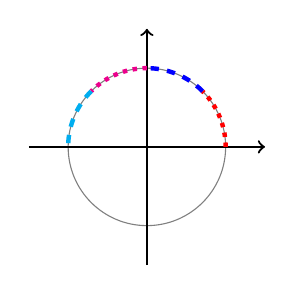
\begin{tikzpicture}
        [scale=1.,
        inner sep=0.5mm,
        pd/.style={circle,draw=red!50,fill=red!20,thick},
        hc/.style={circle,draw=blue!50,fill=blue!20,thick}]
        
        %draw unit circle
        \node (uni_circle1) at (0,0) {};
        \draw[black!50, thin] ($(uni_circle1)$) circle [radius=1];
        \draw[black, thick, ->] ($(uni_circle1)+(-1.5,0)$) -- ($(uni_circle1)+(1.5,0)$);%xaxis
        \draw[black, thick, ->] ($(uni_circle1)+(0,-1.5)$) -- ($(uni_circle1)+(0,1.5)$);%yaxis       

        \draw [dotted, ultra thick,red,domain=0:45] plot ({cos(\x)}, {sin(\x)});
        \draw [dashed, ultra thick,blue,domain=45:90] plot ({cos(\x)}, {sin(\x)});
        \draw [dotted, ultra thick,magenta,domain=90:135] plot ({cos(\x)}, {sin(\x)});
        \draw [dashed, ultra thick,cyan,domain=135:180] plot ({cos(\x)}, {sin(\x)});

        
    \end{tikzpicture}
    \caption{Hypothesis to separate multiple groups of data using the sinusoid projection. The example considers $C=4$.}
    \label{future_work:fig:multi_label_sinusoid}
\end{figure}


\section*{Limitations} While sinusoidal projections have limits, our findings show they retain critical discriminatory structure; according to our experiments, \textit{raw} and \textit{stft} EEG views show limited predictive performance on alternative neurological diseases, including for the classification of Alzheimer's and Parkinson's diseases, thus challenging their use as proxies for fMRI-based diagnostics; the synthesized fMRI is only as good as the quality of paired EEG-fMRI records used to train the model. The addressed problem is binary classification and adapting the methodology to a multinonmial setting requires minor changes. This can be done by detailing angular interval encoding strategies.

\hl{A direct comparison between synthesized and real fMRI requires simultaneously acquired data; for our EEG-only classification cohort no paired fMRI exists, so reconstruction fidelity cannot be measured there, which is precisely the deployment scenario the method targets. The fidelity of the synthesis model itself was established on simultaneous data (NODDI) in }\cite{calhas2022eeg}\hl{ (RMSE $0.3972 \pm 0.0186$, SSIM $0.4613 \pm 0.0198$, best among compared baselines); the present work assesses the downstream diagnostic and interpretive value of the resulting view.}


\section*{Social impact}

Synthesized neuroimaging using EEG offers a scalable, low-cost alternative for mental health diagnostics, potentially improving access across diverse populations. However, ethical concerns include risks from unvalidated synthetic data, privacy issues, and potential misuse. While this study used publicly available, consented datasets, real-world use demands rigorous clinical validation and secure data governance. Environmental impact is also a concern; thus, energy-efficient, low-resource AI methods are encouraged.


\subsection*{Ethics statement}

All procedures performed in this study involving human participants were in accordance with the ethical standards of the institutional and/or national research committee and with the 1964 Helsinki Declaration and its later amendments or comparable ethical standards. The research was conducted in compliance with relevant laws and institutional guidelines.

This study involved the secondary analysis of anonymized data from two primary sources:
\begin{itemize}
    \item Fribourg Dataset: Collected by \citet{dataset2022fribourg} with ethics commmittee approval ID 054/13-CER-FR;
    \item NODDI Dataset: Collected by \citet{dataset_01} with ethics commmittee approval ID ID:4290/001.
\end{itemize}

\bibliographystyle{unsrtnat}
%\bibliography{references}
\begin{thebibliography}{57}
\providecommand{\natexlab}[1]{#1}
\providecommand{\url}[1]{\texttt{#1}}
\expandafter\ifx\csname urlstyle\endcsname\relax
  \providecommand{\doi}[1]{doi: #1}\else
  \providecommand{\doi}{doi: \begingroup \urlstyle{rm}\Url}\fi

\bibitem[Saha et~al.(2005)]{saha2005systematic}
Sukanta Saha et~al.
\newblock A systematic review of the prevalence of schizophrenia.
\newblock \emph{PLoS medicine}, 2005.

\bibitem[Andreou et~al.(2020)]{andreou2020structural}
Christina Andreou et~al.
\newblock Structural and functional imaging markers for susceptibility to psychosis.
\newblock \emph{Molecular psychiatry}, 2020.

\bibitem[Neale et~al.(2015)]{neale2015genetic}
Benjamin~M Neale et~al.
\newblock Genetic analysis of schizophrenia and bipolar disorder reveals polygenicity but also suggests new directions for molecular interrogation.
\newblock \emph{Current opinion in neurobiology}, 2015.

\bibitem[Corcoran et~al.(2020)]{corcoran2020language}
Cheryl~M Corcoran et~al.
\newblock Language as a biomarker for psychosis: {A} natural language processing approach.
\newblock \emph{Schizophrenia research}, 2020.

\bibitem[TAN et~al.(2016)]{tan2016eeg}
O{\u{g}}uz TAN et~al.
\newblock Eeg complexity and frequency in chronic residual schizophrenia.
\newblock \emph{Anatolian Journal of Psychiatry/Anadolu Psikiyatri Dergisi}, 2016.

\bibitem[Ayd{\i}n et~al.(2018)]{aydin2018cortical}
Serap Ayd{\i}n et~al.
\newblock Cortical correlations in wavelet domain for estimation of emotional dysfunctions.
\newblock \emph{Neural Computing and Applications}, 2018.

\bibitem[Oh et~al.(2020)]{oh2020identifying}
Jihoon Oh et~al.
\newblock Identifying schizophrenia using structural {MRI} with a deep learning algorithm.
\newblock \emph{Frontiers in psychiatry}, 2020.

\bibitem[Velakoulis et~al.(2006)]{velakoulis2006hippocampal}
Dennis Velakoulis et~al.
\newblock Hippocampal and amygdala volumes according to psychosis stage and diagnosis: {A} magnetic resonance imaging study of chronic schizophrenia, first-episode psychosis, and ultra--high-risk individuals.
\newblock \emph{Archives of general psychiatry}, 2006.

\bibitem[Haukvik et~al.(2013)]{haukvik2013schizophrenia}
Unn~Kristin Haukvik et~al.
\newblock Schizophrenia--what does structural {MRI} show?
\newblock \emph{Tidsskrift for Den norske legeforening}, 2013.

\bibitem[Ogbole et~al.(2018)]{ogbole2018survey}
Godwin~Inalegwu Ogbole et~al.
\newblock Survey of magnetic resonance imaging availability in {W}est {A}frica.
\newblock \emph{Pan African Medical Journal}, 2018.

\bibitem[Sikka et~al.(2018)]{sikka2018mri}
Apoorva Sikka et~al.
\newblock {MRI} to {FDG}-{PET}: {C}ross-modal synthesis using 3{D} {U}-{N}et for multi-modal {A}lzheimer’s classification.
\newblock In \emph{International Workshop on Simulation and Synthesis in Medical Imaging}, 2018.

\bibitem[Santini et~al.(2020)]{santini2020unpaired}
Gianmarco Santini et~al.
\newblock Unpaired {PET}/{CT} image synthesis of liver region using {C}ycle{GAN}.
\newblock In \emph{16th International Symposium on Medical Information Processing and Analysis}, 2020.

\bibitem[Yang et~al.(2018)]{yang2018mri}
Qianye Yang et~al.
\newblock {MRI} cross-modality neuroimage-to-neuroimage translation.
\newblock \emph{arXiv}, 2018.

\bibitem[Abreu et~al.(2018)]{abreu2018eeg}
Rodolfo Abreu et~al.
\newblock {EEG} synchronization measures predict epilepsy-related {BOLD}-f{MRI} fluctuations better than commonly used univariate metrics.
\newblock \emph{Clinical {N}europhysiology}, 2018.

\bibitem[Daly et~al.(2019)]{daly2019electroencephalography}
Ian Daly et~al.
\newblock Electroencephalography reflects the activity of sub-cortical brain regions during approach-withdrawal behaviour while listening to music.
\newblock \emph{Scientific reports}, 2019.

\bibitem[Liu et~al.(2019)]{liu2019convolutional}
Xueqing Liu et~al.
\newblock A convolutional neural network for transcoding simultaneously acquired {EEG}-f{MRI} data.
\newblock In \emph{NER}, 2019.

\bibitem[Liu et~al.(2020)]{liu2020latent}
Xueqing Liu et~al.
\newblock Latent neural source recovery via transcoding of simultaneous {EEG}-f{MRI}.
\newblock \emph{arXiv}, 2020.

\bibitem[Bricman et~al.(2021)]{bricman2021eeg2fmri}
Paul Bricman et~al.
\newblock {EEG}2f{MRI}: {C}ross-{M}odal {S}ynthesis for {F}unctional {N}euroimaging.
\newblock \emph{Github}, 2021.

\bibitem[Calhas et~al.(2023)]{calhas2022eeg}
David Calhas et~al.
\newblock Eeg to fmri synthesis benefits from attentional graphs of electrode relationships.
\newblock \emph{MLHC}, 2023.

\bibitem[Mehta et~al.(2025)]{mehta2025time}
Neil Mehta et~al.
\newblock Time-varying {EEG} spectral power predicts evoked and spontaneous f{MRI} motor brain activity.
\newblock \emph{arXiv}, 2025.

\bibitem[Li et~al.(2024)]{li2024neurobolt}
Yamin Li et~al.
\newblock Neurobolt: Resting-state {EEG}-to-f{MRI} synthesis with multi-dimensional feature mapping.
\newblock \emph{Advances in Neural Information Processing Systems}, 2024.

\bibitem[Roos et~al.(2025)]{roos2025brainwaves}
Kristofer~Grover Roos et~al.
\newblock From {B}rainwaves to {B}rain {S}cans: {A} {R}obust {N}eural {N}etwork for {EEG}-to-f{MRI} {S}ynthesis.
\newblock \emph{arXiv}, 2025.

\bibitem[Govaert et~al.(2008)]{govaert2008block}
G{\'e}rard Govaert et~al.
\newblock Block clustering with {B}ernoulli mixture models: {C}omparison of different approaches.
\newblock \emph{Computational Statistics \& Data Analysis}, 2008.

\bibitem[Treviso et~al.(2020)]{treviso2020explanation}
Marcos~V Treviso et~al.
\newblock The explanation game: {T}owards prediction explainability through sparse communication.
\newblock \emph{arXiv}, 2020.

\bibitem[Huang et~al.(2020)]{huang2020temporal}
Zirui Huang et~al.
\newblock Temporal circuit of macroscale dynamic brain activity supports human consciousness.
\newblock \emph{Science advances}, 2020.

\bibitem[Tatum~IV(2021)]{tatum2021handbook}
William~O Tatum~IV.
\newblock \emph{Handbook of {EEG} interpretation}.
\newblock Springer Publishing, 2021.

\bibitem[de~Beeck et~al.(2019)]{de2019introduction}
Hans~Op de~Beeck et~al.
\newblock \emph{Introduction to human neuroimaging}.
\newblock Cambridge University Press, 2019.

\bibitem[Oh et~al.(2019)]{oh2019deep}
Shu~Lih Oh et~al.
\newblock Deep convolutional neural network model for automated diagnosis of schizophrenia using eeg signals.
\newblock \emph{Applied Sciences}, 2019.

\bibitem[Barros et~al.(2021)]{barros2021advanced}
Carla Barros et~al.
\newblock Advanced eeg-based learning approaches to predict schizophrenia: Promises and pitfalls.
\newblock \emph{Artificial intelligence in medicine}, 114:\penalty0 102039, 2021.

\bibitem[Fingelkurts et~al.(2007)]{fingelkurts2007impaired}
Andrew~A Fingelkurts et~al.
\newblock Impaired functional connectivity at {EEG} alpha and theta frequency bands in major depression.
\newblock \emph{Human brain mapping}, 2007.

\bibitem[Burgess et~al.(2002)]{burgess2002functional}
Adrian~P Burgess et~al.
\newblock Functional connectivity of gamma {EEG} activity is modulated at low frequency during conscious recollection.
\newblock \emph{International {J}ournal of {{P}}sychophysiology}, 2002.

\bibitem[Albrecht et~al.(2018)]{albrecht2018time}
Matthew~A Albrecht et~al.
\newblock Time and frequency dependent changes in resting state {EEG} functional connectivity following lipopolysaccharide challenge in rats.
\newblock \emph{PLoS One}, 2018.

\bibitem[Roach et~al.(2008)]{roach2008event}
Brian~J Roach et~al.
\newblock Event-related {EEG} time-frequency analysis: {A}n overview of measures and an analysis of early gamma band phase locking in schizophrenia.
\newblock \emph{Schizophrenia bulletin}, 2008.

\bibitem[Bates et~al.(2009)]{bates2009low}
Alan~T Bates et~al.
\newblock Low-frequency {EEG} oscillations associated with information processing in schizophrenia.
\newblock \emph{Schizophrenia research}, 2009.

\bibitem[Bracewell et~al.(1986)]{bracewell1986fourier}
Ronald~Newbold Bracewell et~al.
\newblock \emph{The {F}ourier transform and its applications}.
\newblock McGraw-Hill New York, 1986.

\bibitem[Jacobsen et~al.(2003)]{jacobsen2003sliding}
Eric Jacobsen et~al.
\newblock The sliding {DFT}.
\newblock \emph{{IEEE} Signal Processing Magazine}, 2003.

\bibitem[He et~al.(2016)]{he2016deep}
Kaiming He et~al.
\newblock Deep residual learning for image recognition.
\newblock In \emph{CVPR}, 2016.

\bibitem[Rahimi et~al.(2007)]{rahimi2007random}
Ali Rahimi et~al.
\newblock Random {F}eatures for {L}arge-{S}cale {K}ernel {M}achines.
\newblock In \emph{NIPS}, 2007.

\bibitem[Tancik et~al.(2020)]{tancik2020fourier}
Matthew Tancik et~al.
\newblock Fourier features let networks learn high frequency functions in low dimensional domains.
\newblock \emph{arXiv}, 2020.

\bibitem[Padée et~al.(2022)]{dataset2022fribourg}
Anna Padée et~al.
\newblock "fribourg {U}ltimatum {G}ame in {S}chizophrenia {S}tudy", 2022.

\bibitem[Deligianni et~al.(2014)]{dataset_01}
Fani Deligianni et~al.
\newblock Relating resting-state f{MRI} and {EEG} whole-brain connectomes across frequency bands.
\newblock \emph{Frontiers in Neuroscience}, 2014.

\bibitem[Ba et~al.(2016)]{ba2016layer}
Jimmy~Lei Ba et~al.
\newblock Layer normalization.
\newblock \emph{ar{X}iv}, 2016.

\bibitem[Horat et~al.(2018)]{horat2018impaired}
Sibylle~K Horat et~al.
\newblock Impaired social cognition in schizophrenia during the ultimatum game: An eeg study.
\newblock \emph{Schizophrenia research}, 2018.

\bibitem[Snoek et~al.(2012)]{snoek2012practical}
Jasper Snoek et~al.
\newblock Practical bayesian optimization of machine learning algorithms.
\newblock \emph{NIPS}, 2012.

\bibitem[Kingma et~al.(2014)]{kingma2014adam}
Diederik~P Kingma et~al.
\newblock Adam: {A} method for stochastic optimization.
\newblock \emph{arXiv}, 2014.

\bibitem[Henriques et~al.(2017)]{henriques2017bicpams}
Rui Henriques et~al.
\newblock Bic{PAMS}: {S}oftware for biological data analysis with pattern-based biclustering.
\newblock \emph{BMC bioinformatics}, 2017.

\bibitem[Henriques et~al.(2014)]{henriques2014bicpam}
Rui Henriques et~al.
\newblock Bic{PAM}: {P}attern-based biclustering for biomedical data analysis.
\newblock \emph{Algorithms for Molecular Biology}, 2014.

\bibitem[Castanho et~al.(2022)]{castanho2022biclustering}
Eduardo~N Castanho et~al.
\newblock Biclustering fmri time series: a comparative study.
\newblock \emph{BMC bioinformatics}, 23\penalty0 (1):\penalty0 1--30, 2022.

\bibitem[Pfurtscheller et~al.(1999)]{pfurtscheller1999event}
Gert Pfurtscheller et~al.
\newblock Event-related eeg/meg synchronization and desynchronization: basic principles.
\newblock \emph{Clinical neurophysiology}, 110\penalty0 (11):\penalty0 1842--1857, 1999.

\bibitem[Itil(1977)]{itil1977qualitative}
Turan~M Itil.
\newblock Qualitative and quantitative eeg findings in schizophrenia.
\newblock \emph{Schizophrenia bulletin}, 1977.

\bibitem[Neyshabur et~al.(2015)]{neyshabur2015path}
Behnam Neyshabur et~al.
\newblock Path-{SGD}: {P}ath-normalized optimization in deep neural networks.
\newblock \emph{NIPS}, 2015.

\bibitem[Yadav et~al.(2019)]{yadav2019patients}
Ajay~Kumar Yadav et~al.
\newblock Patients understanding of their diagnosis and treatment plans during discharge in emergency ward in a tertiary care centre: a qualitative study.
\newblock \emph{JNMA: Journal of the Nepal Medical Association}, 2019.

\bibitem[Sui et~al.(2018)]{sui2018multimodal}
Jing Sui et~al.
\newblock Multimodal neuromarkers in schizophrenia via cognition-guided {MRI} fusion.
\newblock \emph{Nature communications}, 2018.

\bibitem[de~Filippis et~al.(2019)]{de2019machine}
Renato de~Filippis et~al.
\newblock Machine learning techniques in a structural and functional {MRI} diagnostic approach in schizophrenia: {A} systematic review.
\newblock \emph{Neuropsychiatric disease and treatment}, 2019.

\bibitem[Chin et~al.(2018)]{chin2018recognition}
Rowena Chin et~al.
\newblock Recognition of schizophrenia with regularized support vector machine and sequential region of interest selection using structural magnetic resonance imaging.
\newblock \emph{Scientific Reports}, 2018.

\bibitem[Cetin-Karayumak et~al.(2020)]{cetin2020white}
Suheyla Cetin-Karayumak et~al.
\newblock White matter abnormalities across the lifespan of schizophrenia: a harmonized multi-site diffusion {MRI} study.
\newblock \emph{Molecular psychiatry}, 2020.

\bibitem[Pinto et~al.(2022)]{pinto2022interpretable}
Mauro Pinto et~al.
\newblock Interpretable {EEG} seizure prediction using a multiobjective evolutionary algorithm.
\newblock \emph{Scientific reports}, 2022.

\end{thebibliography}

\normalsize


\clearpage
\newpage
\appendix

\begin{proof}
Let $\phi(z) = \left[ \cos(\omega_1^\top z + \beta_1), \dots, \cos(\omega_d^\top z + \beta_d) \right]$, where each $\omega_i \sim \mathcal{N}(0, I_d)$ and $\beta_i \sim \mathrm{Uniform}[0, 2\pi]$. The inner product between projected vectors is:
\[
\phi(z_1)^\top \phi(z_2) = \sum_{i=1}^d \cos(\omega_i^\top z_1 + \beta_i) \cos(\omega_i^\top z_2 + \beta_i).
\]
Using the trigonometric identity:
\[
\cos(a)\cos(b) = \frac{1}{2}[\cos(a - b) + \cos(a + b)],
\]
we write:
\begin{align*}
    &\cos(\omega_i^\top z_1 + \beta_i) \cos(\omega_i^\top z_2 + \beta_i) = \\
&\frac{1}{2} \left[ \cos(\omega_i^\top(z_1 - z_2)) + \cos(\omega_i^\top(z_1 + z_2) + 2\beta_i) \right].    
\end{align*}


Taking the expectation over $\beta_i \sim \mathrm{Uniform}[0, 2\pi]$, the second term vanishes:
\[
\mathbb{E}_{\beta_i}[\cos(\omega_i^\top(z_1 + z_2) + 2\beta_i)] = 0.
\]

Thus,
\[
\mathbb{E}_{\omega, \beta}[\phi(z_1)^\top \phi(z_2)] = \frac{1}{2} \sum_{i=1}^d \mathbb{E}_{\omega_i}[\cos(\omega_i^\top(z_1 - z_2))].
\]

Let $\delta = z_1 - z_2$. Since $\omega_i^\top \delta \sim \mathcal{N}(0, \|\delta\|_2^2)$, we use the identity:
\[
\mathbb{E}_{x \sim \mathcal{N}(0, \sigma^2)}[\cos(x)] = e^{-\frac{1}{2}\sigma^2},
\]
to obtain:
\[
\mathbb{E}_{\omega_i}[\cos(\omega_i^\top \delta)] = e^{-\frac{1}{2}\|\delta\|_2^2}.
\]

Putting it together:
\[
\mathbb{E}_{\omega, \beta}[\phi(z_1)^\top \phi(z_2)] = \frac{d}{2} e^{-\frac{1}{2}\|z_1 - z_2\|_2^2}.
\]

Therefore, for any $\|z_1 - z_2\|_2 > 0$, we have:
\[
\mathbb{E}_{\omega, \beta}[\phi(z_1)^\top \phi(z_2)] < \frac{d}{2} < d,
\]
proving the result.
\end{proof}

\clearpage
\newpage

\end{document}